\documentclass[pdflatex,sn-mathphys-num]{sn-jnl}

\usepackage{graphicx}%
\usepackage{multirow}%
\usepackage{amsmath,amssymb,amsfonts}%
\usepackage{amsthm}%
\usepackage{mathrsfs}%
\usepackage[title]{appendix}%
\usepackage{xcolor}%
\usepackage{textcomp}%
\usepackage{manyfoot}%
\usepackage{booktabs}%
\usepackage{algorithm}%
\usepackage{algorithmicx}%
\usepackage{algpseudocode}%
\usepackage{listings}%

\lstdefinestyle{bashstyle}{
    language=bash,
    basicstyle=\ttfamily\small,
    keywordstyle=\color{blue}\bfseries,
    commentstyle=\color{gray},
    stringstyle=\color{orange},
    morekeywords={mkdir, cd, cmake, ninja},
    backgroundcolor=\color{lightgray!20},
    frame=single,
    breaklines=true,
    showstringspaces=false,
    columns=fullflexible
}


\lstdefinestyle{fileresultstyle}{
    basicstyle=\ttfamily\small,
    numbers=left,
    numberstyle=\tiny,
    stepnumber=1,
    numbersep=8pt,
    breaklines=true,
    breakatwhitespace=false,
    showstringspaces=false,
    backgroundcolor=\color{lightgray!20},
    frame=single,
    columns=fullflexible
}

\lstdefinestyle{pythonstyle}{
    language=Python,
    basicstyle=\ttfamily\small,
    keywordstyle=\color{blue}\bfseries,
    commentstyle=\color{gray}\itshape,
    stringstyle=\color{orange},
    numbers=left,
    numberstyle=\tiny,
    stepnumber=1,
    numbersep=8pt,
    backgroundcolor=\color{lightgray!20},
    frame=single,
    breaklines=true,
    breakatwhitespace=false,
    showstringspaces=false,
    columns=fullflexible
}

\begin{document}

\title[Operation Cybershadow]{Operation Cybershadow}

\author*{\fnm{David} \sur{Dudas}}\email{david.dudas03@e-uvt.ro}

\affil{\orgdiv{Faculty of Mathematics and Computer Science},
       \orgname{West University of Timisoara},
       \orgaddress{\city{Timisoara},
                   \country{Romania}}}

\abstract{This paper present the operation CYBERSHADOW\@: A Digital Whodunit. This operation is about a digital forensics
investigation triggered by an infiltration of the Ministry of Strategic Technologies. This paper presents four chapters
that describe the investigation, the tools used, and the findings.}

\keywords{Cybersecurity, Digital Forensics, Investigation, C++}

\maketitle

\section{Introduction}\label{introduction}

\par This paper tends to present operation CYBERSHADOW\@: A Digital Whoduint that started at InterSec Division HQ.

\par The Ministry of Strategic Technologies was inflitrated by an unknown actor and the only clues left are a
compromised machine, garbled traffic logs, a suspicious USB image, and a stash of potentially synthetic media.

\par In the following sections I will present how I approached the problem, what tools I used, and what I found.

\subsection{Chapter 1: Shadows in the File System}\label{chapter1_introduction}

\par The investigation begins with a laptop with a compressed archive on its drive. This archive contains a web of
directories and files that may contain clues. The filenames and types are misleading, so we will need a script that can
recursively scan a folder and identify the actual file types.

\par The script should be designed for the Windows operating system and I will write it in C++.

\par The script will offer a command line interface with the following options:

\begin{itemize}
    \item \texttt{-i} or \texttt{--input} followed by a path: Specify the input file path.
    \item \texttt{-s} or \texttt{--sigs} followed by a path: Specify the file type map path.
    \item \texttt{-d} or \texttt{--depth} followed by a number: Specify the search depth (when input path is a directory).
    \item \texttt{-h} or \texttt{--help}: Display the help message.
\end{itemize}

\par We can use this script to scan the archive and identify the actual file types.

\subsection{Chapter 2: Listening to Ghosts}

\par A machine started acting strange after the user installed something searching for Google Authenticator.
There are two separate LAN segments, each tainted by infection. We will analyze the traffic for each.

\subsubsection{Operation MOONFALL\@: The False Authenticator}

\par The infection took root after accessing a fake Google Authenticator page. In order to find out \textbf{infected Windows
client's IP address, MAC address, host name} and also the \textbf{likely domain name used by the fake Authenticator site and
the Command and Control (C2) server IP address}, we will analyze the traffic logs.

\subsubsection{Operation GREENWIRE\@: The Domain Breach}

\par There are some outbound connections to obscure hosts, odd DNS behavior, and encrypted chatter in a different AD
environment. Seems to be a different malware strain, but it might be linked to the previous analysis.

\par Here we are interested in finding out the \textbf{IP adddress and host name} of the infected Windows machine,
the associated \textbf{user account names}, the responsible \textbf{malware family}, the \textbf{exact UTC timestamp}
when the infection began, and the \textbf{domain name} used within this AD environment.

\subsection{Chapter 3: Echoes from the Drive}\label{chapter3_introduction}

\par An USB device is next clue. I wat profesionally wiped, but the imaging team was able to extract a complete forensic
dump: IMAGE.ISO\@.

\par We also know that there is a file inside the image that was encrypted using a 2-byte XOR cipher, the archives may
be nested within the image, and one file is believed to be an image (BMP, PNG, or JPG), but it also be more than just
pixels.

\par I will try to \textbf{recover} all the extractable files from the ISO image, \textbf{classify} them by type with
as much accuracy as possible, decrypt the encrypted file, and examine image files.

\subsection{Chapter 4: Faces Behind the Curtain}

\par There is also a folder that has surfaced during the investigation. It contains dozens of images and videos
depicting high-ranking officials in scenarios that could ignite international crises. However, there is something
suspicious about them.

\par I will analyze the media files and will try to \textbf{determine which images and videos are authentic and which
have been manipulated}.

\section{Methodology}

\subsection{File Type Detection Script}\label{ftds}

\par In this section, I will present the C++ program used to detect the file types from the achive from chapter~\ref{chapter1_introduction}.

\par I will use the magic number of the file's headers to determine the file type. The magic number is a unique sequence
of bytes at the beginning of a file that identifies its type. I will use Gary Kessler's magic number list\cite{filesigs}
for this.

\par The program reads the json file using the nlohmann::json library\cite{nlohmann_json} and populates a map where
the magic number is the key and the file type details are the value. The program then recursively scans the input
directory and reads the first eight bytes of each file. It checks if the magic number is present in the map and prints
the file type details if it is found.

\par The program won't work if the input path and the signatures path are not provided. The depth is optional \-- if not
provided, the program will scan the entire directory tree.

\par To compile the program, you need to have a C++ compiler, cmake, and optionally ninja installed. You can use the
following commands to compile the program:

\begin{lstlisting}[style=bashstyle]
mkdir build
cd build
cmake -G Ninja ..
ninja
\end{lstlisting}

\par This will produce and executable file named \texttt{stdf.exe} and a test file named \texttt{stdf\_tests.exe} in the
\texttt{build} directory. However, if you do not want to compile the program, the executable files are also available in
the \texttt{bin} directory of the repository.

\subsection{Network Traffic Analysis}

\subsubsection{The False Authenticator}\label{tfa}

\par This investigation will focus on a pcap file that contains the traffic logs from the infected machine. The goal is
to find out the likely domain name used by the fake Authenticator site, the infected Windows client's IP address,host
name, and MAC address, and the C2 IP address.

\par To find out the \textbf{domain name} of the fake Authenticator site, I will look for DNS queries. Since I know that
the domain name contains the word `moon', I will filter the DNS queries for that keyword.

\par The \textbf{infected Windows client's IP address} can be found by looking at the source IP address of the DNS event.

\par The pcap file also contains some \textbf{NBNS} traffic, which can be used to find the \textbf{host name} of the
infected machine. I will need to look for NBNS queries and responses that contain the infected machine's IP address.
Also, these NBNS queries will contain the \textbf{MAC address} in the \textbf{Etherned II} header. 

\par In order to find the \textbf{Command and Control (C2) IP address}, I will look for http, udp, and tcp traffic, only
in external communication for the infected machine's IP address.

\subsubsection{The Domanin Breach}\label{tdb}

\par During the investigation of this pcap file, I will focus on finding the AD enviroment's domain name, the malware
family, the infected Windows machine's IP address and host name, the exact UTC timestamp when the infection began and
the user account names associated with this incident.

\par I know that the AD environment's domain name contains the word `green', so I will filter the DNS queries for that
keyword.

\par To identify the \textbf{malware family}, I will look for suspicious traffic patterns and analyze the payloads of
the packets.

\par The infected Windows machine's IP address and host name can be found after identifying the malware family. When I
will find the malware, I will be able to identify the infected machine's IP address. The host name can be found in the
NBNS queries and responses, similar to the previous investigation.

\par In order to find the \textbf{exact UTC timestamp} when the infection began, I will look for the trigger of the
suspicious traffic.

\par For the \textbf{user account names}, I also need to know the malware family. Once I identify it, I expect to find
the user account names implicated in the infection in the traffic logs.

\subsection{Digital Foresics \& Hidden Data Extraction}\label{dfhde}

\par In this section, I will present how I will try to extract the files from the USB image.

\par The first step is to simply mount the image and copy-paste it's contents. But as we might expect, that's not all.
I will also do some further analysis, deep scan on the extracted files.

\par For the encrypted file, I will simply brute-force the 2-byte XOR key. I will use a python script for that together
with the `file' linux command to identify the decrypted file type. There will be multiple possibilities, however I
excpect that 90\% of the results will be just `data' and I will have to manually check the rest.

\par I will also use the `binwalk` linux command to deep scan every file from the image. For image files (PNG, JPG, etc.),
I will use both `exiftool'\cite{suhardjono2022forensic} and `steghide' to extract the metadata and hidden data.

\subsection{Deepfake Detection}

\par In this section, I need to analyze the media files and determine which images and videos are authentic and which
have been manipulated. For this, I will do manual analysis, but I will also use some tools to help me, such as `exiftool'.

\par In case of images, I will look for pixel structure anomalies, metadata and lighting inconsistencies, thin details
such as hair strands, and other signs of manipulation. I will also use `exiftool' to extract the metadata and check
if the image was edited with a known software.

\par In case of videos, I will look for frame inconsistencies, audio-visual mismatches, irregularities in motion and 
lighting, and other signs of manipulation.

\section{Results}\label{results}

\subsection{File Type Detection Script Results}\label{chapter1_results}

\par We used the File Type Detection Script~\ref{ftds} to scan the archive from chapter ~\ref{chapter1_introduction}.

\begin{lstlisting}[style=bashstyle]
.\bin\stfd.exe -s .\chapter1\resources\file_sigs.json -i <path_to_chapter1_archive>
\end{lstlisting}

\par The output of the following is as follows:

\begin{lstlisting}[style=fileresultstyle]
'chapter1\archives\arch.7z': 7Z (7-Zip compressed file)
'chapter1\archives\ARCH2.bz2': DMG (Mac Disk image (BZ2 compressed))
'chapter1\archives\arch3.zip': XPT (eXact Packager Models)
'chapter1\archives\notes.jar': AVI|CDA|QCP|RMI|WAV|WEBP (Resource Interchange File Format)
'chapter1\docs\Chairing_Guidelines.doc': WPS (MSWorks text document)
'chapter1\docs\Meeting-agenda-template.docx': XPT (eXact Packager Models)
'chapter1\docs\meeting-checklist-template.docx': XPT (eXact Packager Models)
'chapter1\docs\meeting_staff.doc': AVI|CDA|QCP|RMI|WAV|WEBP (Resource Interchange File Format)
'chapter1\docs\more\docs\in\here\How to Survive a meeting.doc': WPS (MSWorks text document)
'chapter1\docs\more\docs\in\here\how-to-conduct-a-meeting-2.docx': XPT (eXact Packager Models)
'chapter1\fun\1711922908449.jpg': SYS (Windows executable)
'chapter1\fun\62fbe39b1c30c95b2cc78f2b_LB0250..png': PNG (PNG image)
'chapter1\fun\AdobeStock_407607989-scaled.jpeg': SYS (Windows executable)
'chapter1\fun\business-meeting.jpg': SYS (Windows executable)
'chapter1\fun\images (1).jpg': SYS (Windows executable)
'chapter1\fun\images.jpg': SYS (Windows executable)
'chapter1\fun\leading-a-meeting-1024x683.jpg.optimal.jpg': SYS (Windows executable)
'chapter1\fun\stock_photo.png': XPT (eXact Packager Models)
'chapter1\fun\types-of-meetings.webp': AVI|CDA|QCP|RMI|WAV|WEBP (Resource Interchange File Format)
'chapter1\music\emotional_music_561.mp3': VXD|386 (Windows virtual device drivers)
'chapter1\music\eona-emotional-ambient-pop-351436.mp3': SYS (Windows executable)
'chapter1\music\future-design-344320.mp3': SYS (Windows executable)
'chapter1\music\jungle-waves-drumampbass-electronic-inspiring-promo-345013.mp3': SYS (Windows executable)
'chapter1\presentations\1 Setup.pptx': XPT (eXact Packager Models)
'chapter1\presentations\AWKUM-offical-PowerPoint-Template.pptx': XPT (eXact Packager Models)
'chapter1\presentations\CCB_MeetingMgmt.ppt': WPS (MSWorks text document)
'chapter1\presentations\Firefighter-Silhouette-PowerPoint-Diagram.pptx': XPT (eXact Packager Models)
'chapter1\presentations\JS2-Mod1.pptx': XPT (eXact Packager Models)
'chapter1\presentations\planning_call_meeting.ppt': VXD|386 (Windows virtual device drivers)
'chapter1\presentations\samplepptx.pptx': XPT (eXact Packager Models)
'chapter1\presentations\slide-zoom-powerpoint-template.pptx': XPT (eXact Packager Models)
'chapter1\unknown\file1': XPT (eXact Packager Models)
'chapter1\unknown\file2': SYS (Windows executable)
'chapter1\unknown\file3': VXD|386 (Windows virtual device drivers)
'chapter1\unknown\file4': VXD|386 (Windows virtual device drivers)
'chapter1\unknown\file5': Unknown
'chapter1\unknown\file6': Unknown
'chapter1\unknown\file7': Unknown
'chapter1\unknown\file8': Unknown
'chapter1\unknown\file9': Unknown
'chapter1\videos\bear_fun.mp4': VXD|386 (Windows virtual device drivers)
'chapter1\videos\COWS_AT_THE_GRASS.mp4': AVIF (High Efficiency Image Container (HEIC)_1)
'chapter1\videos\Good_dog.mp4': AVIF (High Efficiency Image Container (HEIC)_1)
'chapter1\videos\MVI_2350.mov': AVIF (High Efficiency Image Container (HEIC)_1)
'chapter1\videos\waterfall2.avi': AVI|CDA|QCP|RMI|WAV|WEBP (Resource Interchange File Format)
\end{lstlisting}

\subsubsection{The False Authenticator Results}

\par We used the network traffic analysis tools to analyze the pcap file from opeartion MOONFALL~\ref{tfa}.

\par The first step was to filter the DNS queries for the keyword `moon' in order to find the \textbf{likely domain}
name used by the fake Authenticator site. The result was: \texttt{bluemoontuesday.com}.

\par The \textbf{infected Windows client's IP address} was found in the DNS event: \texttt{10.1.17.215}.

\par The \textbf{host name} of the infected machine was found in the NBNS queries' and responses' NetBIOS Name Service:
\texttt{DESKTOP-L8C6GSJ}.

\par The \textbf{MAC address} of the infected machine was found in the NBNS queries' and responses' Ethernet II header:
\texttt{00:d0:b7:26:4a:74}.

\par In order to find the \textbf{Command and Control (C2) IP address}, I looked for http, udp, and tcp traffic, only
in external communication for the infected machine's IP address. There were multiple HTTP GET requests at /1517096937
to an IP address that seems to be the C2 server: \texttt{5.252.153.241}.

\subsubsection{The Domain Breach Results}

\par In the second part of the network traffic analysis, I focused on the pcap file from operation GREENWIRE~\ref{tdb}.

\par The first step was to filter the DNS queries for the keyword `green' in order to find the \textbf{AD environment's
domain name}. The result was: \texttt{fargreentech.com}.

\par While looking for the \textbf{malware family}, I noticed some SMTP traffic with suspicious patterns. Fromt the STMP
traffic, I was able to extract some base64 encoded strings that were usernames and passwords. There were multiple
authentication attempts, some of them successful. Because of the suspicious patterns, I belive that the malware family
is a variant of the \textbf{Emotet malware}\cite{kuraku2020emotet}.

\par All this SMTP traffic was generated by the \textbf{infected Windows machine with IP address} \texttt{10.12.3.66}.
Given the IP address, I was able to find the \textbf{host name} of the infected machine: \texttt{DESKTOP-LUOABV1}.

\par Regarding the \textbf{exact UTC timestamp} when the infection began, I found a suspicious DNS query at 18.742200
(relative to the pcap file's start time) that was made by the infected machine. The query was for the domain name 
\texttt{fargreentech.com}.

\par The \textbf{user account names} associated with this incident were found in the SMTP traffic. The usernames were:

\begin{itemize}
    \item darin.figueroa
    \item marlon.gamba
    \item minami.hinaka
    \item tenpo.kaihatsu
    \item noboyasu.takahashi
    \item elena.chavez
\end{itemize}

\subsubsection{Digital Foresics \& Hidden Data Extraction Results}

\par After mounting the USB image, and copying its contents~\ref{dfhde}, I got 5 files:

\begin{itemize}
    \item \texttt{data1.bin}
    \item \texttt{data2.bin}
    \item \texttt{data3.bin}
    \item \texttt{data4.bin}
    \item \texttt{data5.bin}
\end{itemize}

\par The first step was to see the realy type of each file. I used the `file' linux command to do that. The results were:

\begin{lstlisting}[style=fileresultstyle]
data1.bin: data
data2.bin: 7-zip archive data, version 0.4
data3.bin: PE32+ executable for MS Windows 10.00 (GUI), x86-64, 8 sections
data4.bin: Microsoft Word 2007+
data5.bin: PC bitmap, Windows 3.x format, 1927 x 1080 x 24, image size 6246720, resolution 2835 x 2835 px/m, cbSize 6246774, bits offset 54
\end{lstlisting}

\par As expected~\ref{chapter3_introduction}, there is an encrypted file (\textbf{data1.bin}) for which the `file' command
returned `data'. I wrote the following python script to brute-force the 2-byte XOR key:

\begin{lstlisting}[language=Python, style=pythonstyle]
import itertools
import sys

input_file = "data1.bin"

with open(input_file, "rb") as f:
    data = f.read()

def is_digit(byte):
    return 0x30 <= byte <= 0x39

print("")
for b1 in range(256):
    for b2 in range(256):
        if is_digit(b1) or is_digit(b2):
            print(f"Trying key: {b1:02x}{b2:02x}", end='\r')
            sys.stdout.flush()

            key = bytes([b1, b2])
            
            decrypted = bytearray()
            for i in range(len(data)):
                decrypted.append(data[i] ^ key[i % 2])
            
            output_file = f"o/output_{b1:02x}_{b2:02x}.bin"
            with open(output_file, "wb") as out:
                out.write(decrypted)
            print(f"[+] Saved {output_file} with key {b1:02x}{b2:02x}")
\end{lstlisting}

\par The script saves each attempt to an output file named \texttt{output\_XX\_YY.bin}, where \texttt{XX} and
\texttt{YY} are the
hexadecimal representation of the two bytes of the key.

\par After running the script, I used the `file' command to check the output files. Most of them were just `data', but
for \texttt{0x62 0x30} there was a \textbf{zip archive}.

\par After extracting the zip archive, I found two files:

\begin{itemize}
    \item \texttt{data1.bin}: a simple text file with the content: \texttt{`I'd tell you a joke about a buffer overflow...
        but you might not be able to handle it.\%'}
    \item \texttt{data2.bin}: an image file:
\end{itemize}

\begin{figure}[htbp]
    \centering
    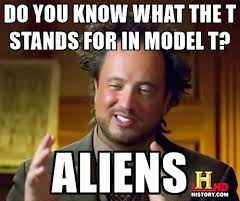
\includegraphics[width=0.5\textwidth]{images/data1_data2.bin.png}
    \caption{The image file extracted from the data1.bin.}
    \label{fig:data1_data2}
\end{figure}

\par For the \textbf{data2.bin} file, since in reality it was a 7zip file, I was able to simply unzip it with
`7z x data2.bin'. The result is another file: \texttt{data1.bin}, that after running the `file' command, I found out
that it is a mpv4 video file about WTF News:

\begin{figure}[htbp]
    \centering
    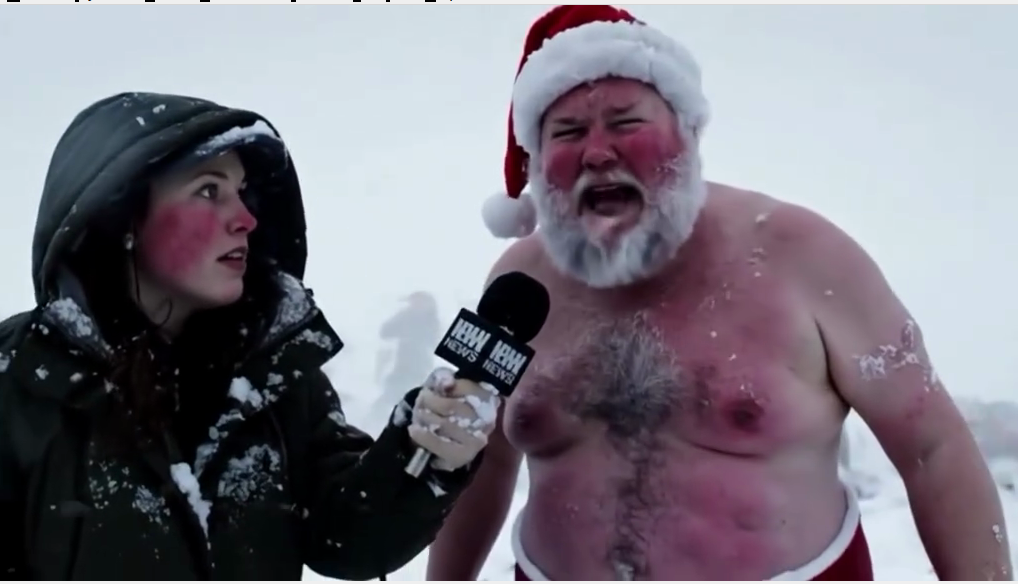
\includegraphics[width=0.5\textwidth]{images/data2.png}
    \caption{A screenshot of the video extracted from the data2.bin file.}
    \label{fig:data2}
\end{figure}

\par The \textbf{data3.bin} file seemed to be a Windows executable, but I tried to run an extrac scan on it using
`binwalk -e data3.bin'. This extracted the following files:

\begin{lstlisting}[style=fileresultstyle]
2C490/image.png
40568/image.png
786A8/image.png
83328/image.png
97400/image.png
A80B8/image.png
BC190/image.png
CE650/image.png
\end{lstlisting}

\begin{figure}[htbp]
    \centering
    
\includegraphics[width=0.22\textwidth]{images/2C490/image.png}
    
\includegraphics[width=0.22\textwidth]{images/40568/image.png}
    
\includegraphics[width=0.22\textwidth]{images/786A8/image.png}
    
\includegraphics[width=0.22\textwidth]{images/83328/image.png} \\[1ex]
    
    
\includegraphics[width=0.22\textwidth]{images/97400/image.png}
    
\includegraphics[width=0.22\textwidth]{images/A80B8/image.png}
    
\includegraphics[width=0.22\textwidth]{images/BC190/image.png}
    
\includegraphics[width=0.22\textwidth]{images/CE650/image.png}
    \label{fig:data3_images}
\end{figure}

\par The \textbf{data4.bin} file was a Microsoft Word 2007+ document. However, I still tried to run `binwalk -e data4.bin'
on it, and it seems like there was also a Microsoft PowerPoint document inside it. The result of the binwalk command was
two folders:

\begin{itemize}
    \item \texttt{0}: the actual Microsoft Word document.
    \item \texttt{9940}: the Microsoft PowerPoint document.
\end{itemize}

\par For \textbf{data5.bin}, I also tried to run `binwalk -e data5.bin' on it, but without any success. I've also tried
`steghide', but still no results. However, after running `zsteg data5.bin', I found the following results:

\begin{itemize}
    \item \textbf{text}: \texttt{`We don't do late submissions... we do denial of service on deadlines.'}
    \item \textbf{file}: \texttt{Targa image data - RGBA 1290 x 514 x 1 +259 +512 - 3-bit alpha `\\001'}
    \item \textbf{file}: \texttt{OpenPGP Public Key}
    \item \textbf{file}: \texttt{Applesoft BASIC program data, first line number 138}
\end{itemize}

\pagebreak

\subsubsection{Deepfake Detection Results}

\par In this section, I will present the results of the deepfake analysis for each media file.

\begin{figure}[htbp]
    \centering
    \begin{tabular}{ccc}
        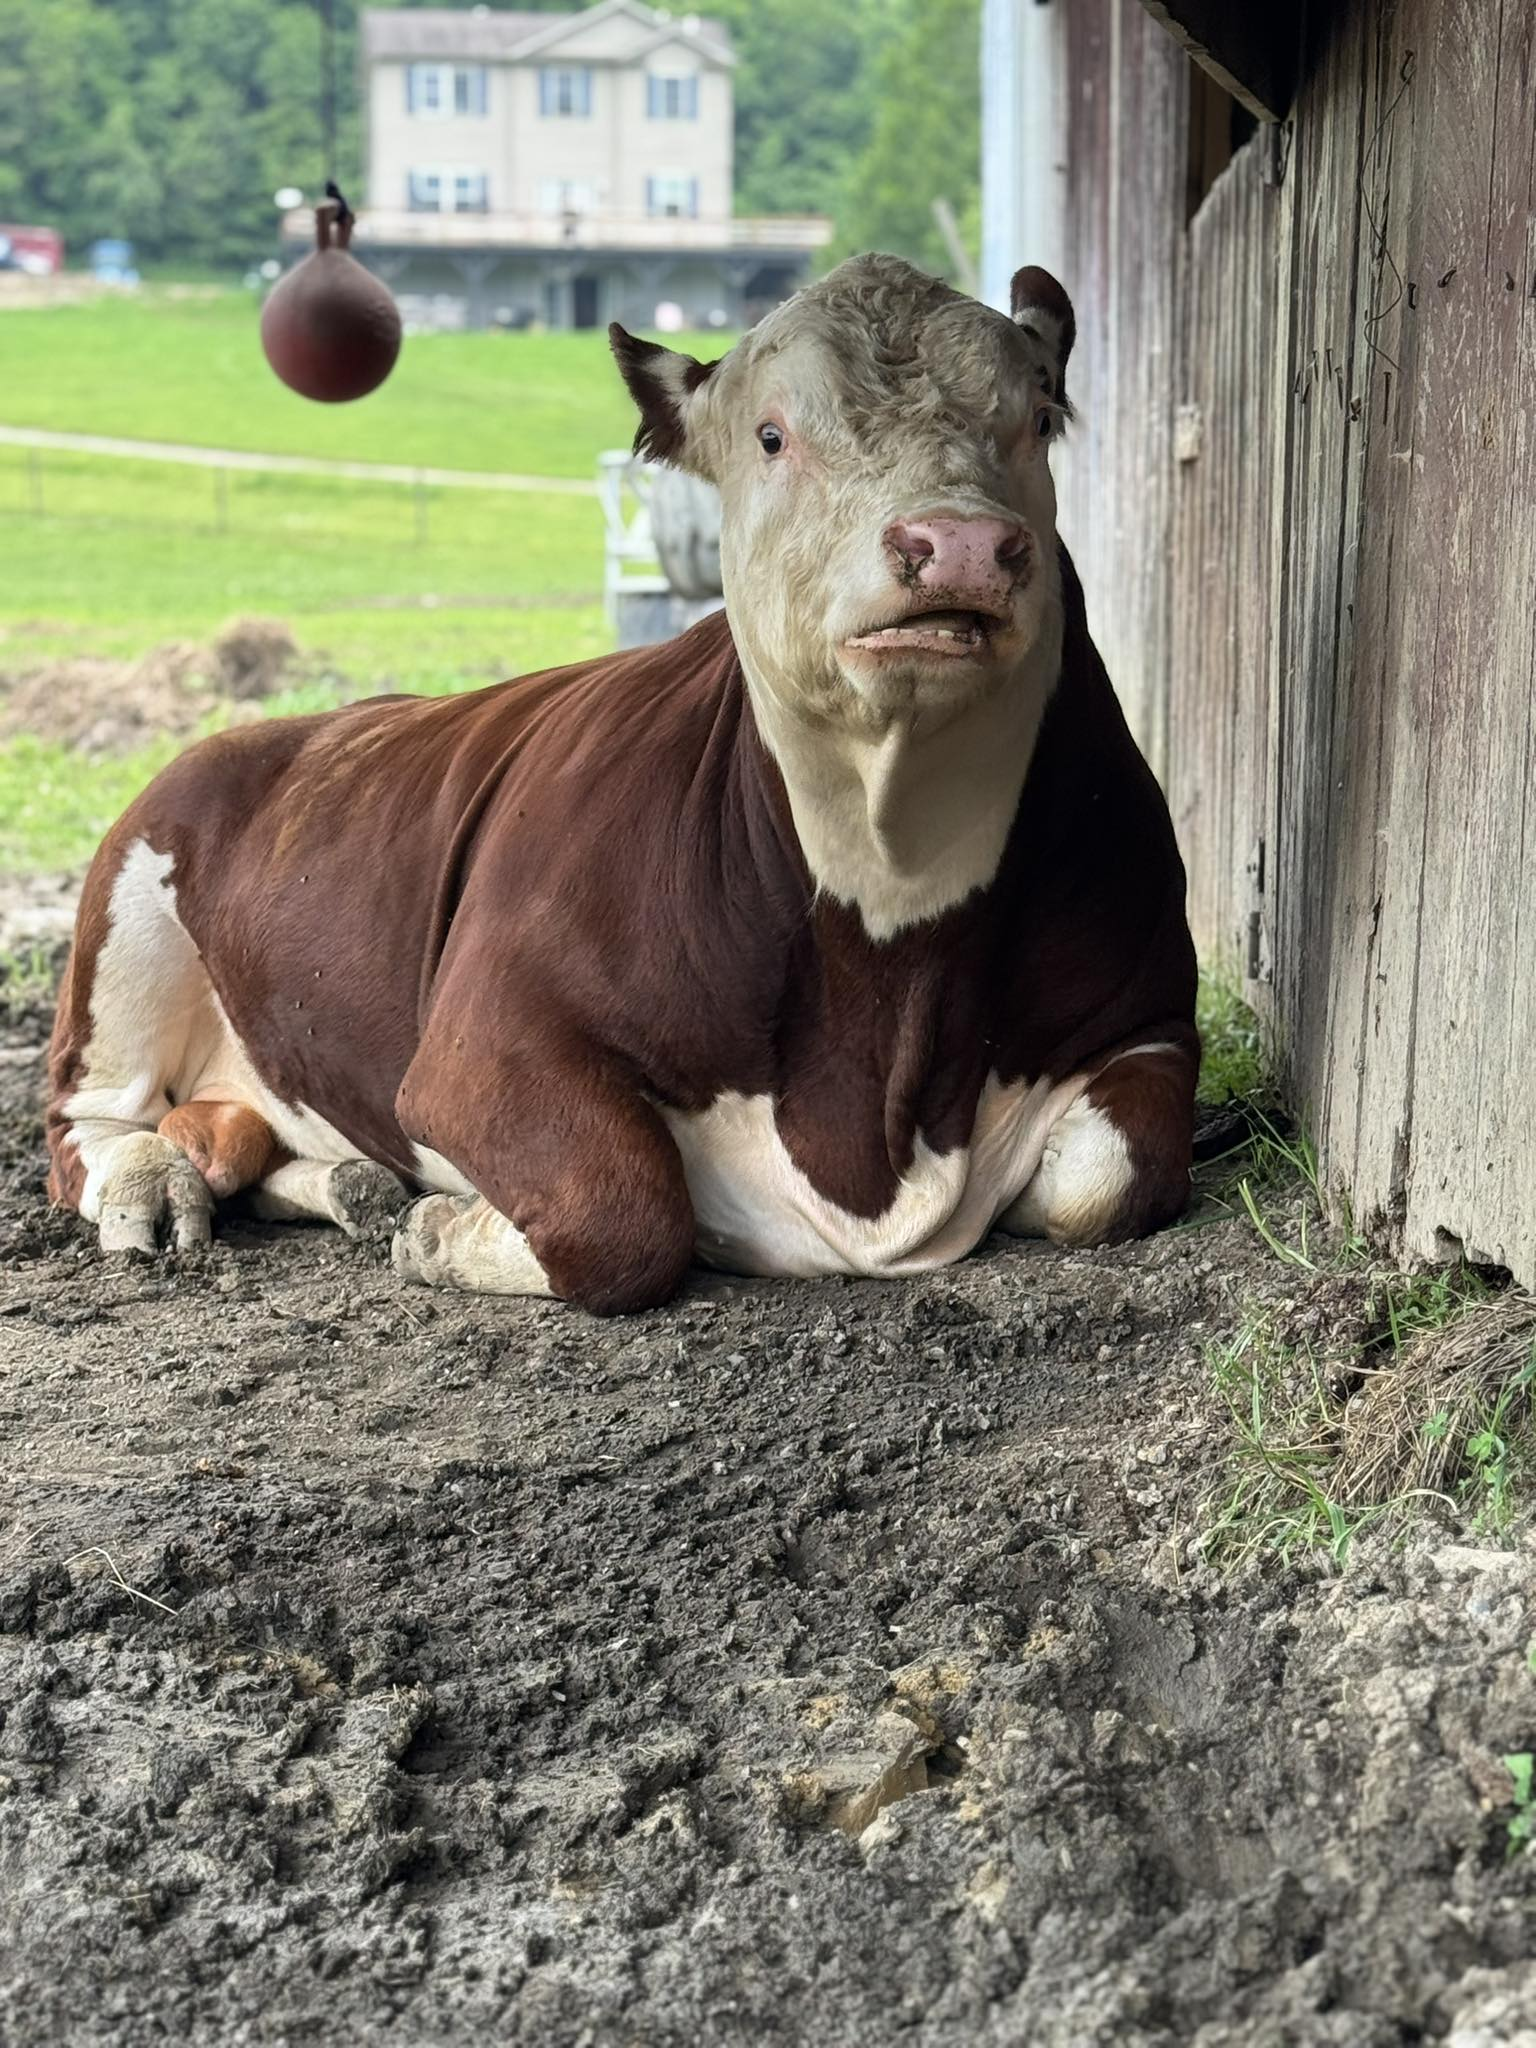
\includegraphics[width=0.3\textwidth]{images/set1/p1.jpg} &
        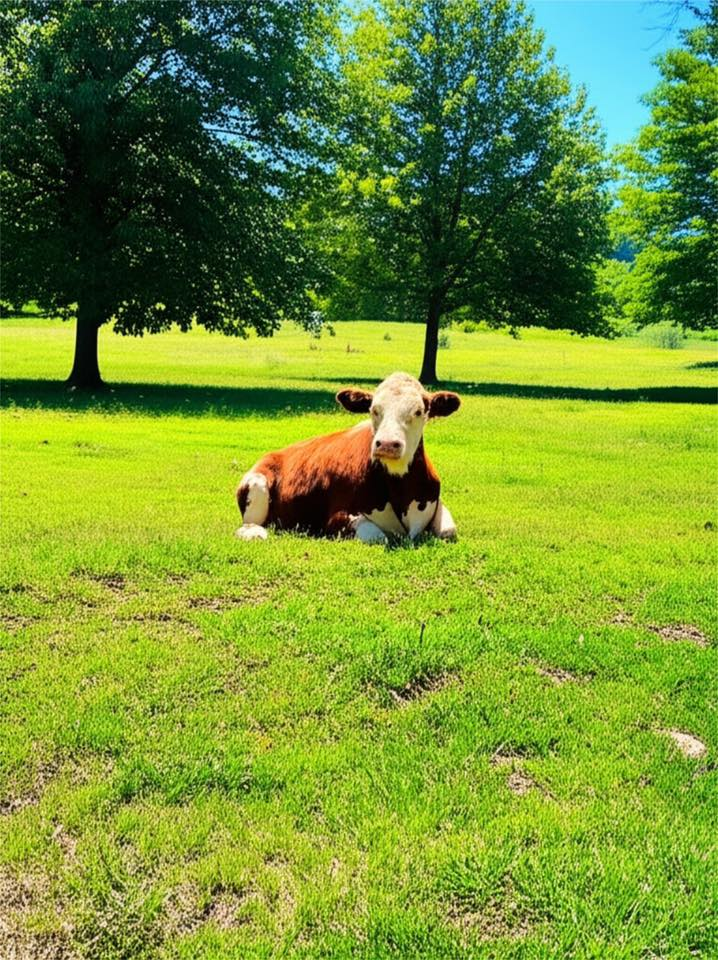
\includegraphics[width=0.3\textwidth]{images/set1/p2.jpg} &
        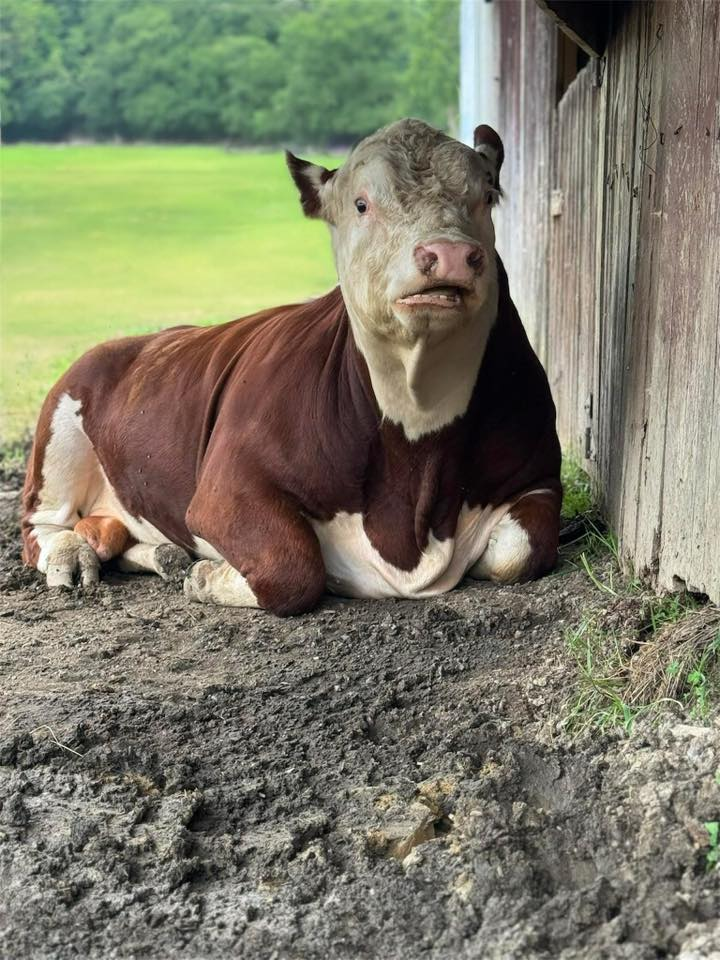
\includegraphics[width=0.3\textwidth]{images/set1/p3.jpg} \\
        set1/p1.jpg & set1/p2.jpg & set1/p3.jpg
    \end{tabular}
    \label{fig:set1_images}
\end{figure}

\par \textbf{set1/p1.jpg} \-- This image appears to be \textbf{authentic}. The pixel structure is consistent, the
lighting is natural, and there are no signs of manipulation.

\par \textbf{set1/p2.jpg} \-- It's really hard to find any inconsistencies or irregularities in hair strands, edges,
lighting, shadows, or pixel structure. Even if some parts in grass, in the tree's leaves, and in the cow's front legs
are a bit strange, I can't tell if this is a result of a manipulation or not.

\par \textbf{set1/p3.jpg} \-- Here it is clearly visible that the edges and the hair strands are not consistent and
they are significantly worse quality. All around the cow there is a blur-ish area that removes the end of the hair
strands, mostly around the cow's ears. This image is \textbf{manipulated}.

\begin{figure}[htbp]
    \centering
    \begin{tabular}{cccc}
        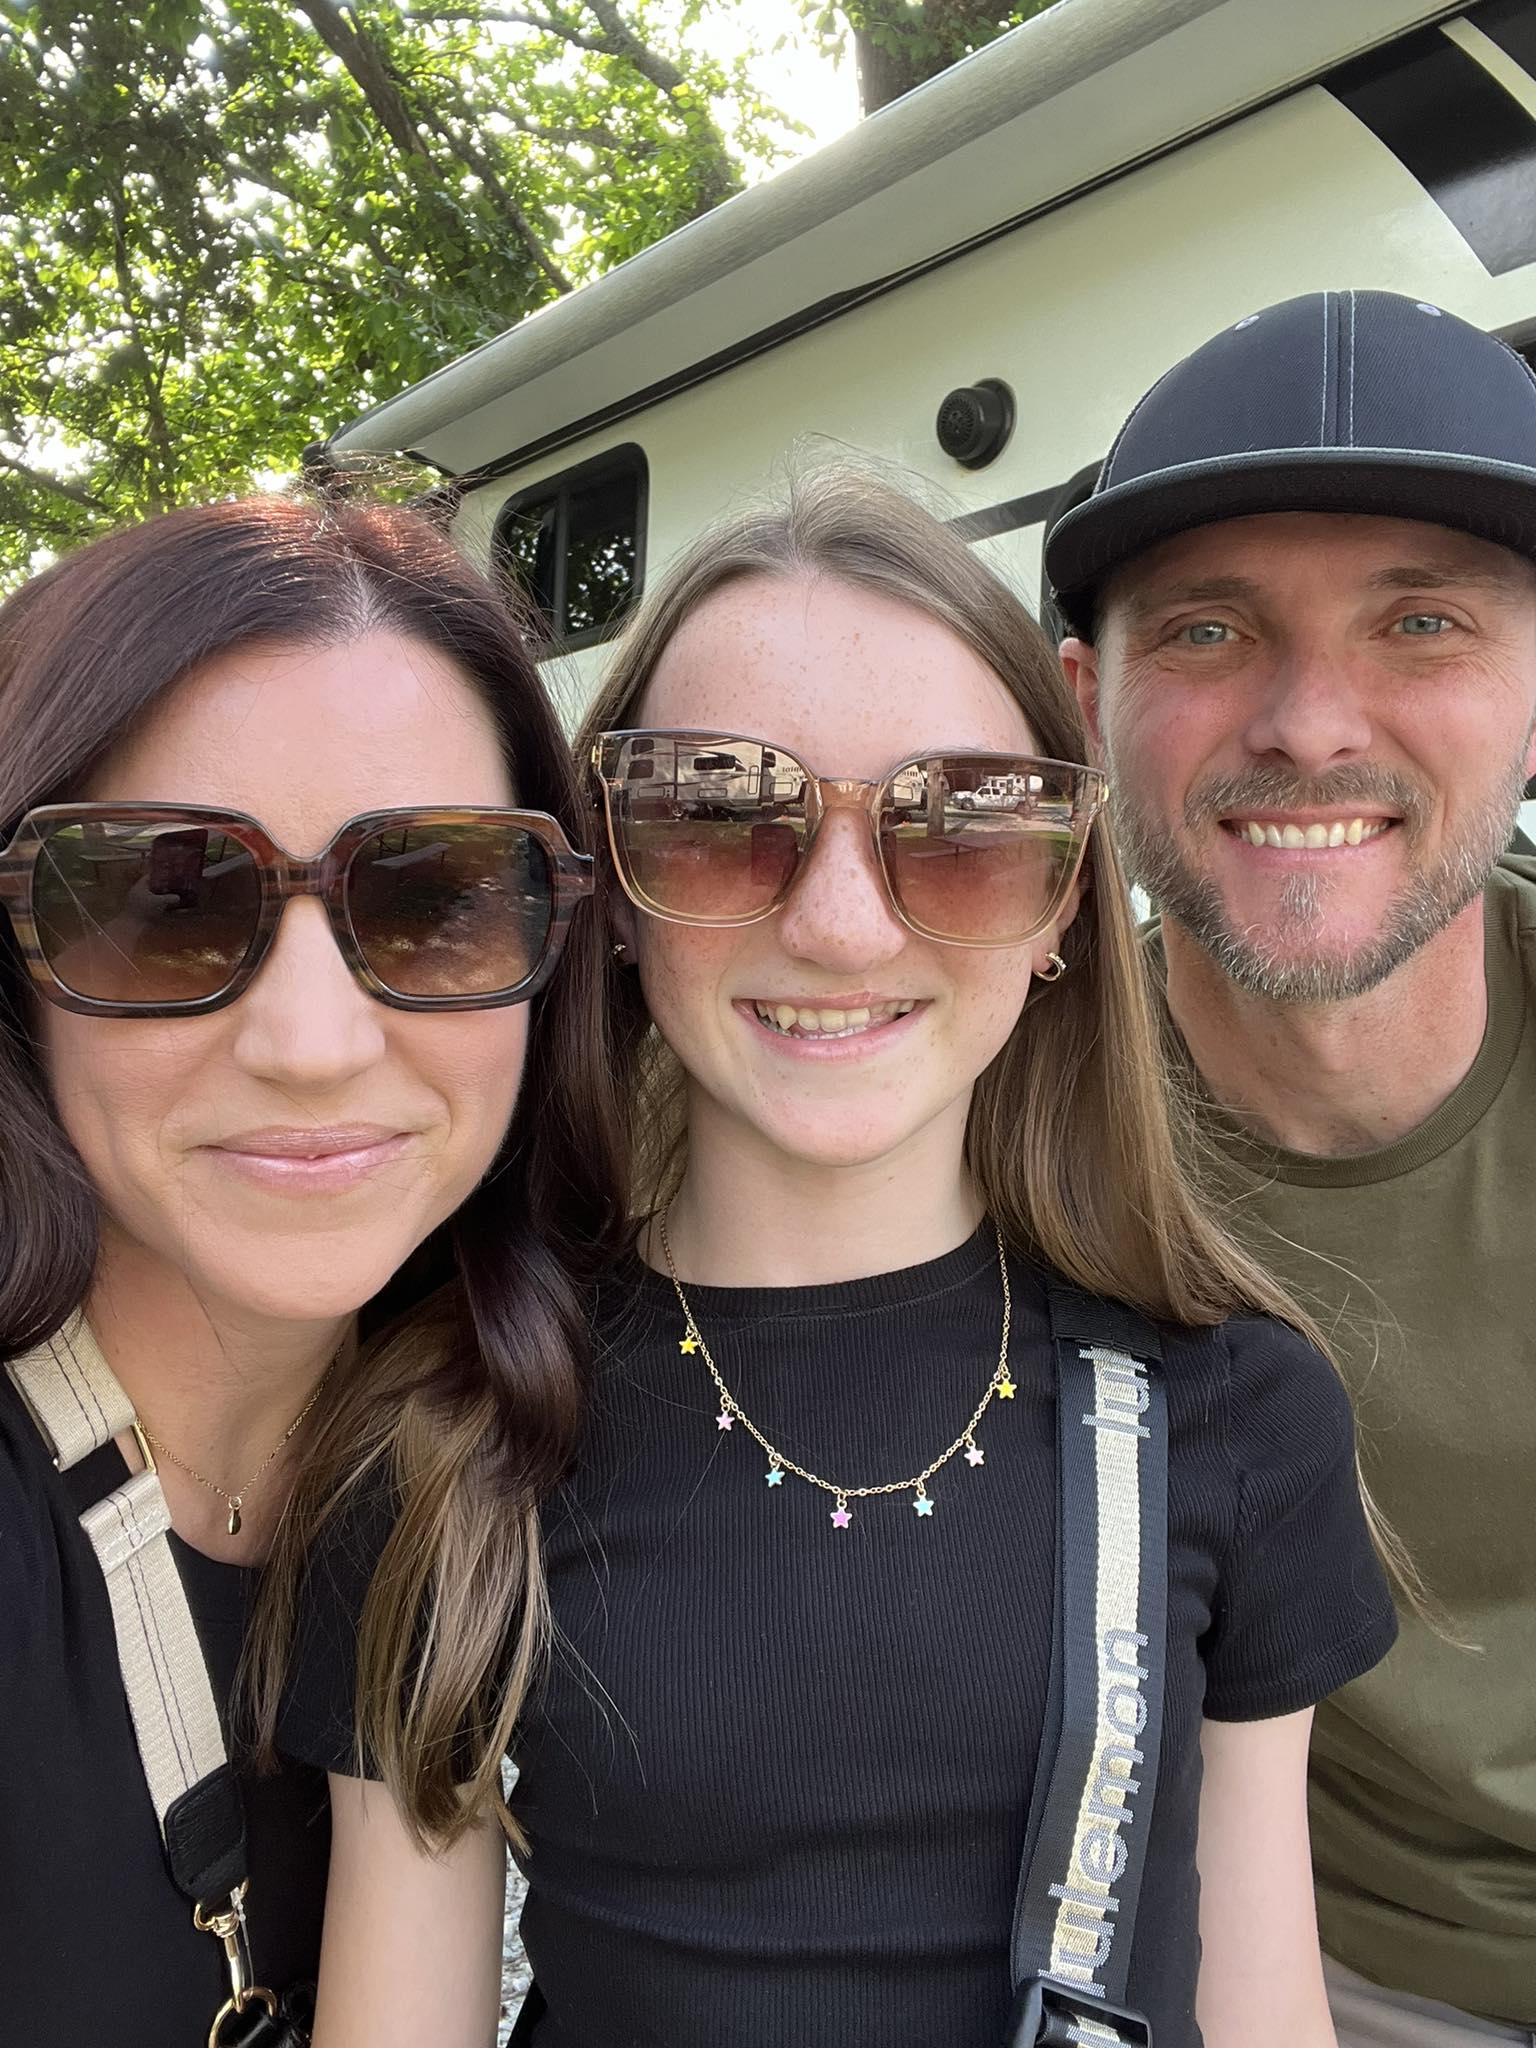
\includegraphics[width=0.3\textwidth]{images/set2/p1.jpg} &
        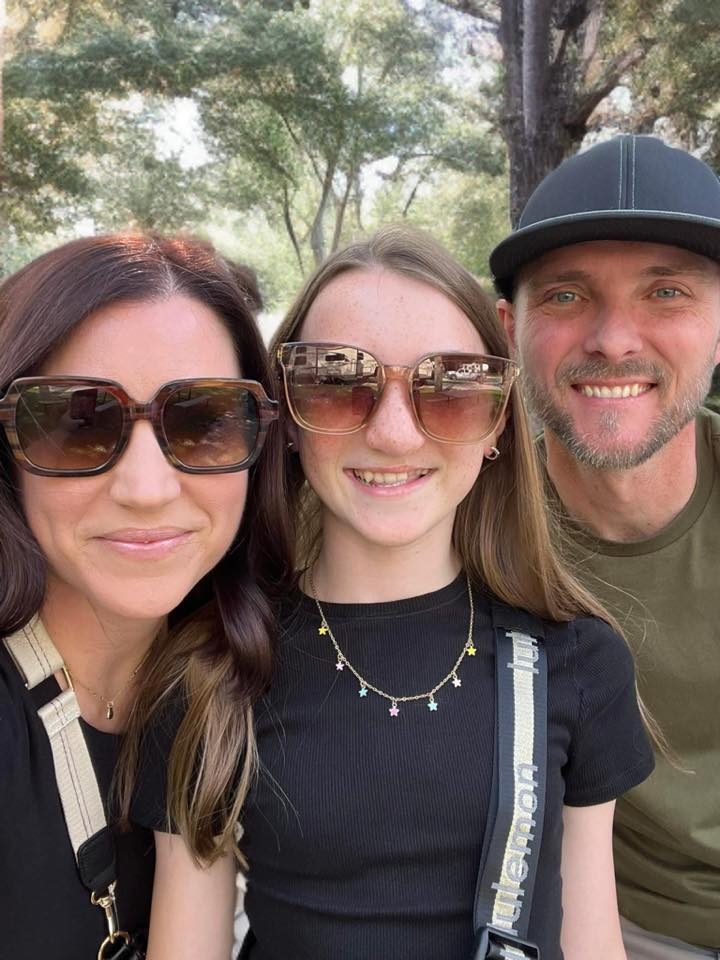
\includegraphics[width=0.3\textwidth]{images/set2/p2.jpg} \\
        set2/p1.jpg & set2/p2.jpg
    \end{tabular}
    \label{fig:set2_images}
\end{figure}

\par \textbf{set2/p1.jpg} \-- It seems like there is nothing wrong with this image. I think it is \textbf{authentic}.

\par \textbf{set2/p2.jpg} \-- Here the hair strands make it obvious that the background was changed. All around the
hair it is really blurry and the end of the hair strands are not visible. This image is \textbf{manipulated}.

\begin{figure}[htbp]
    \centering
    \begin{tabular}{cccc}
        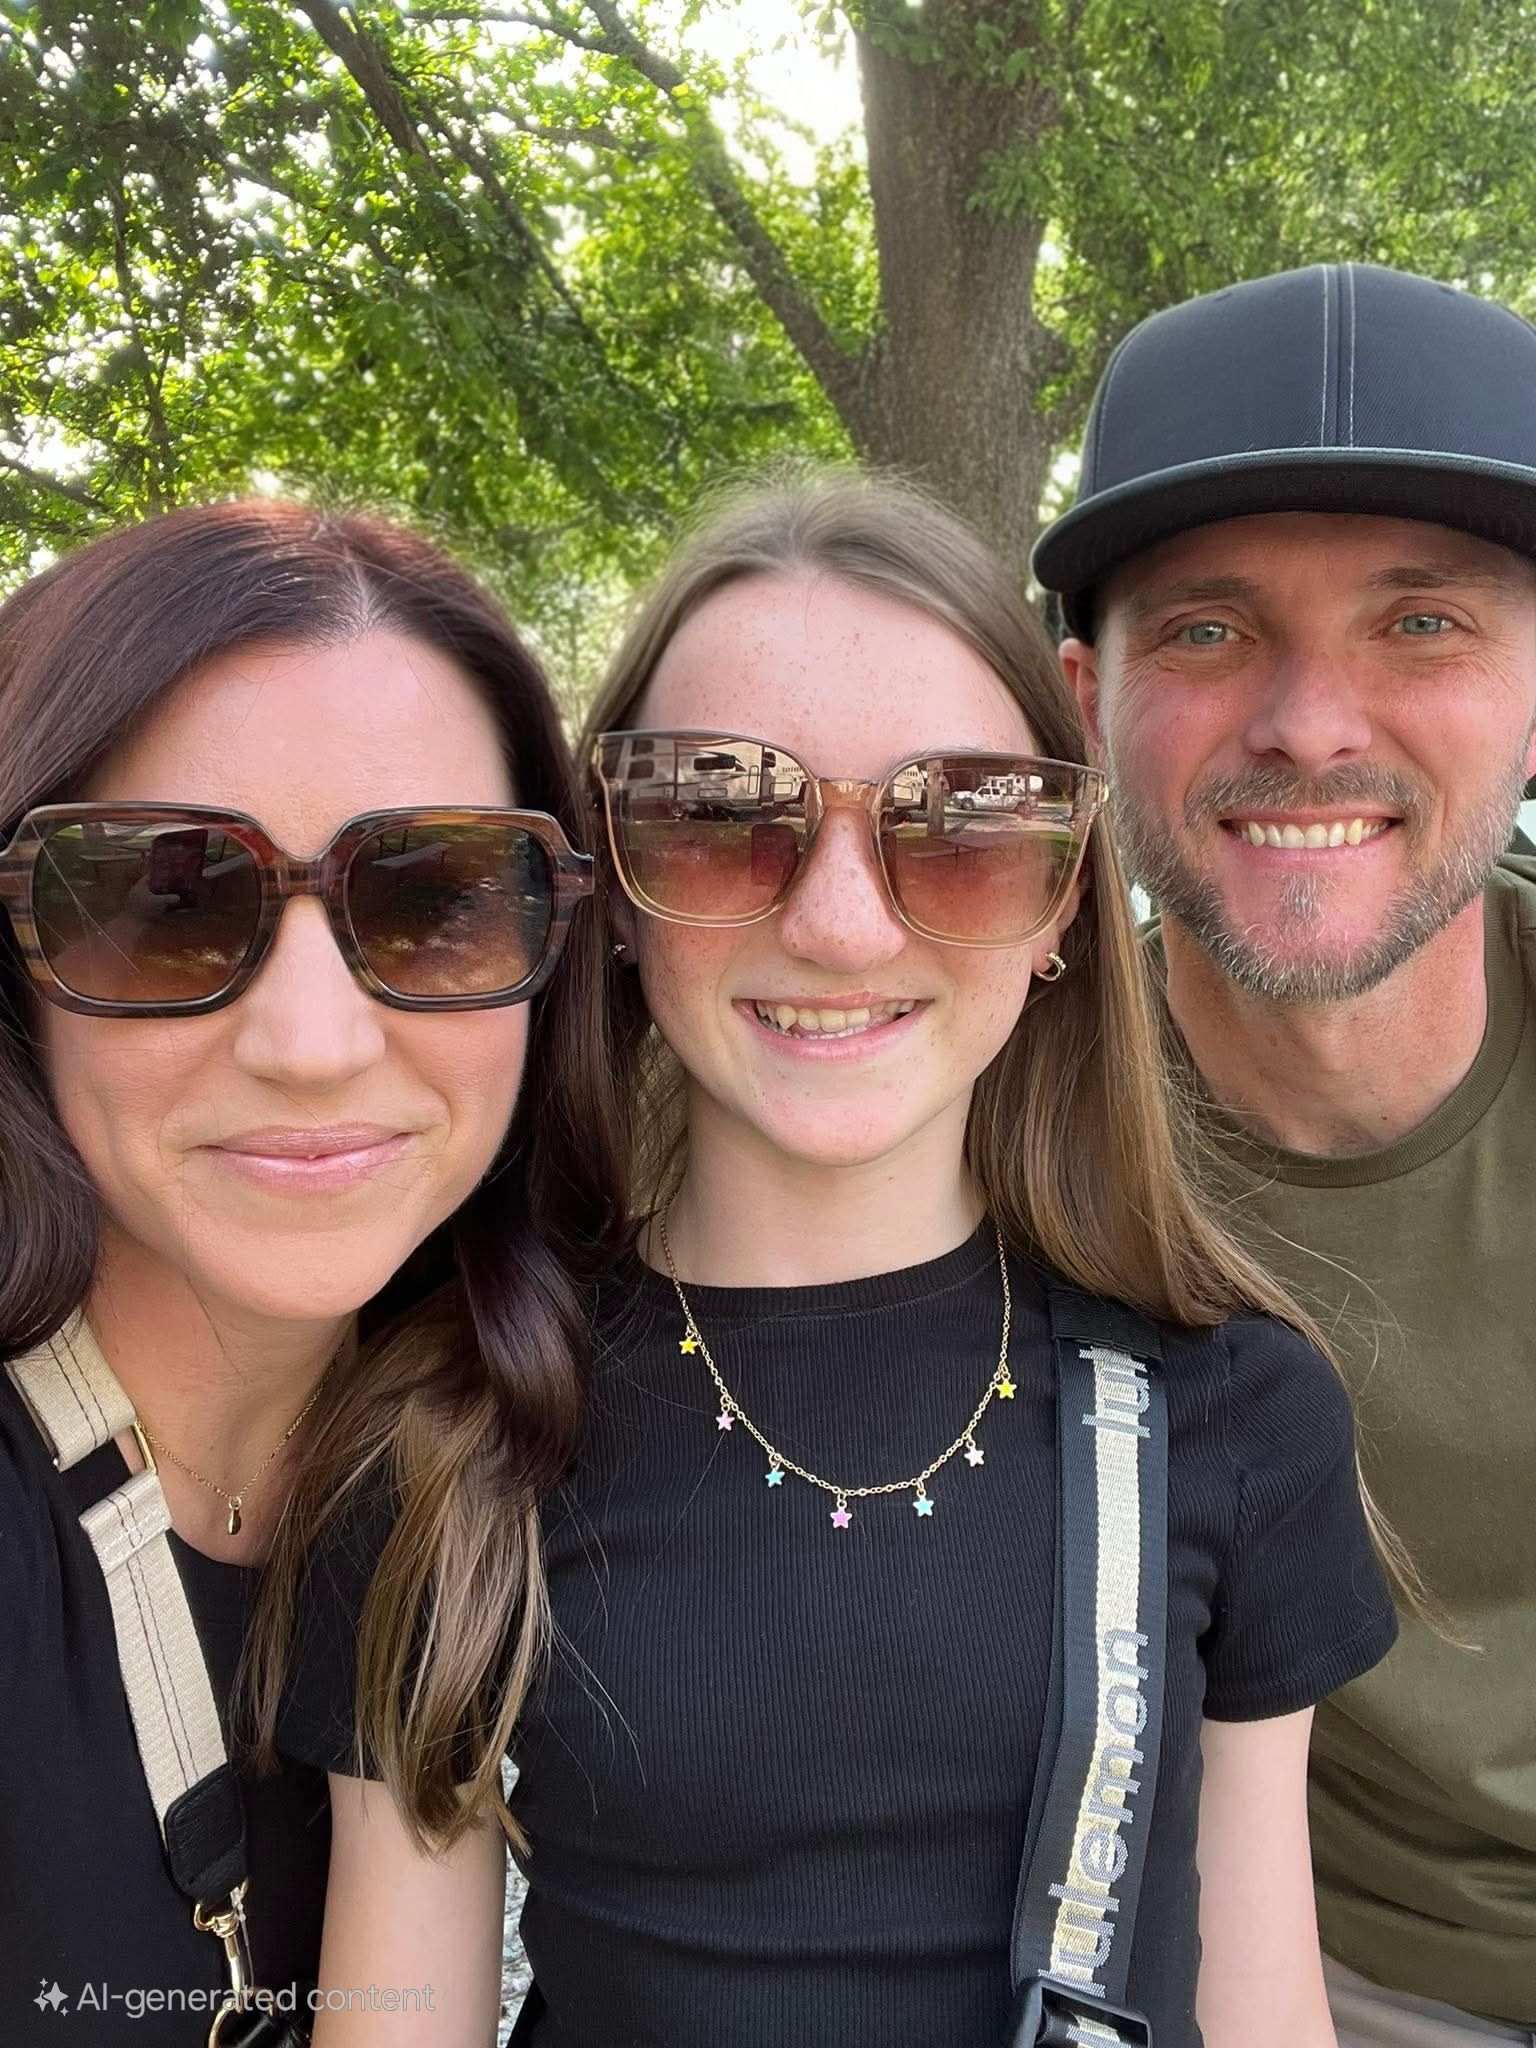
\includegraphics[width=0.3\textwidth]{images/set2/p3.jpg} &
        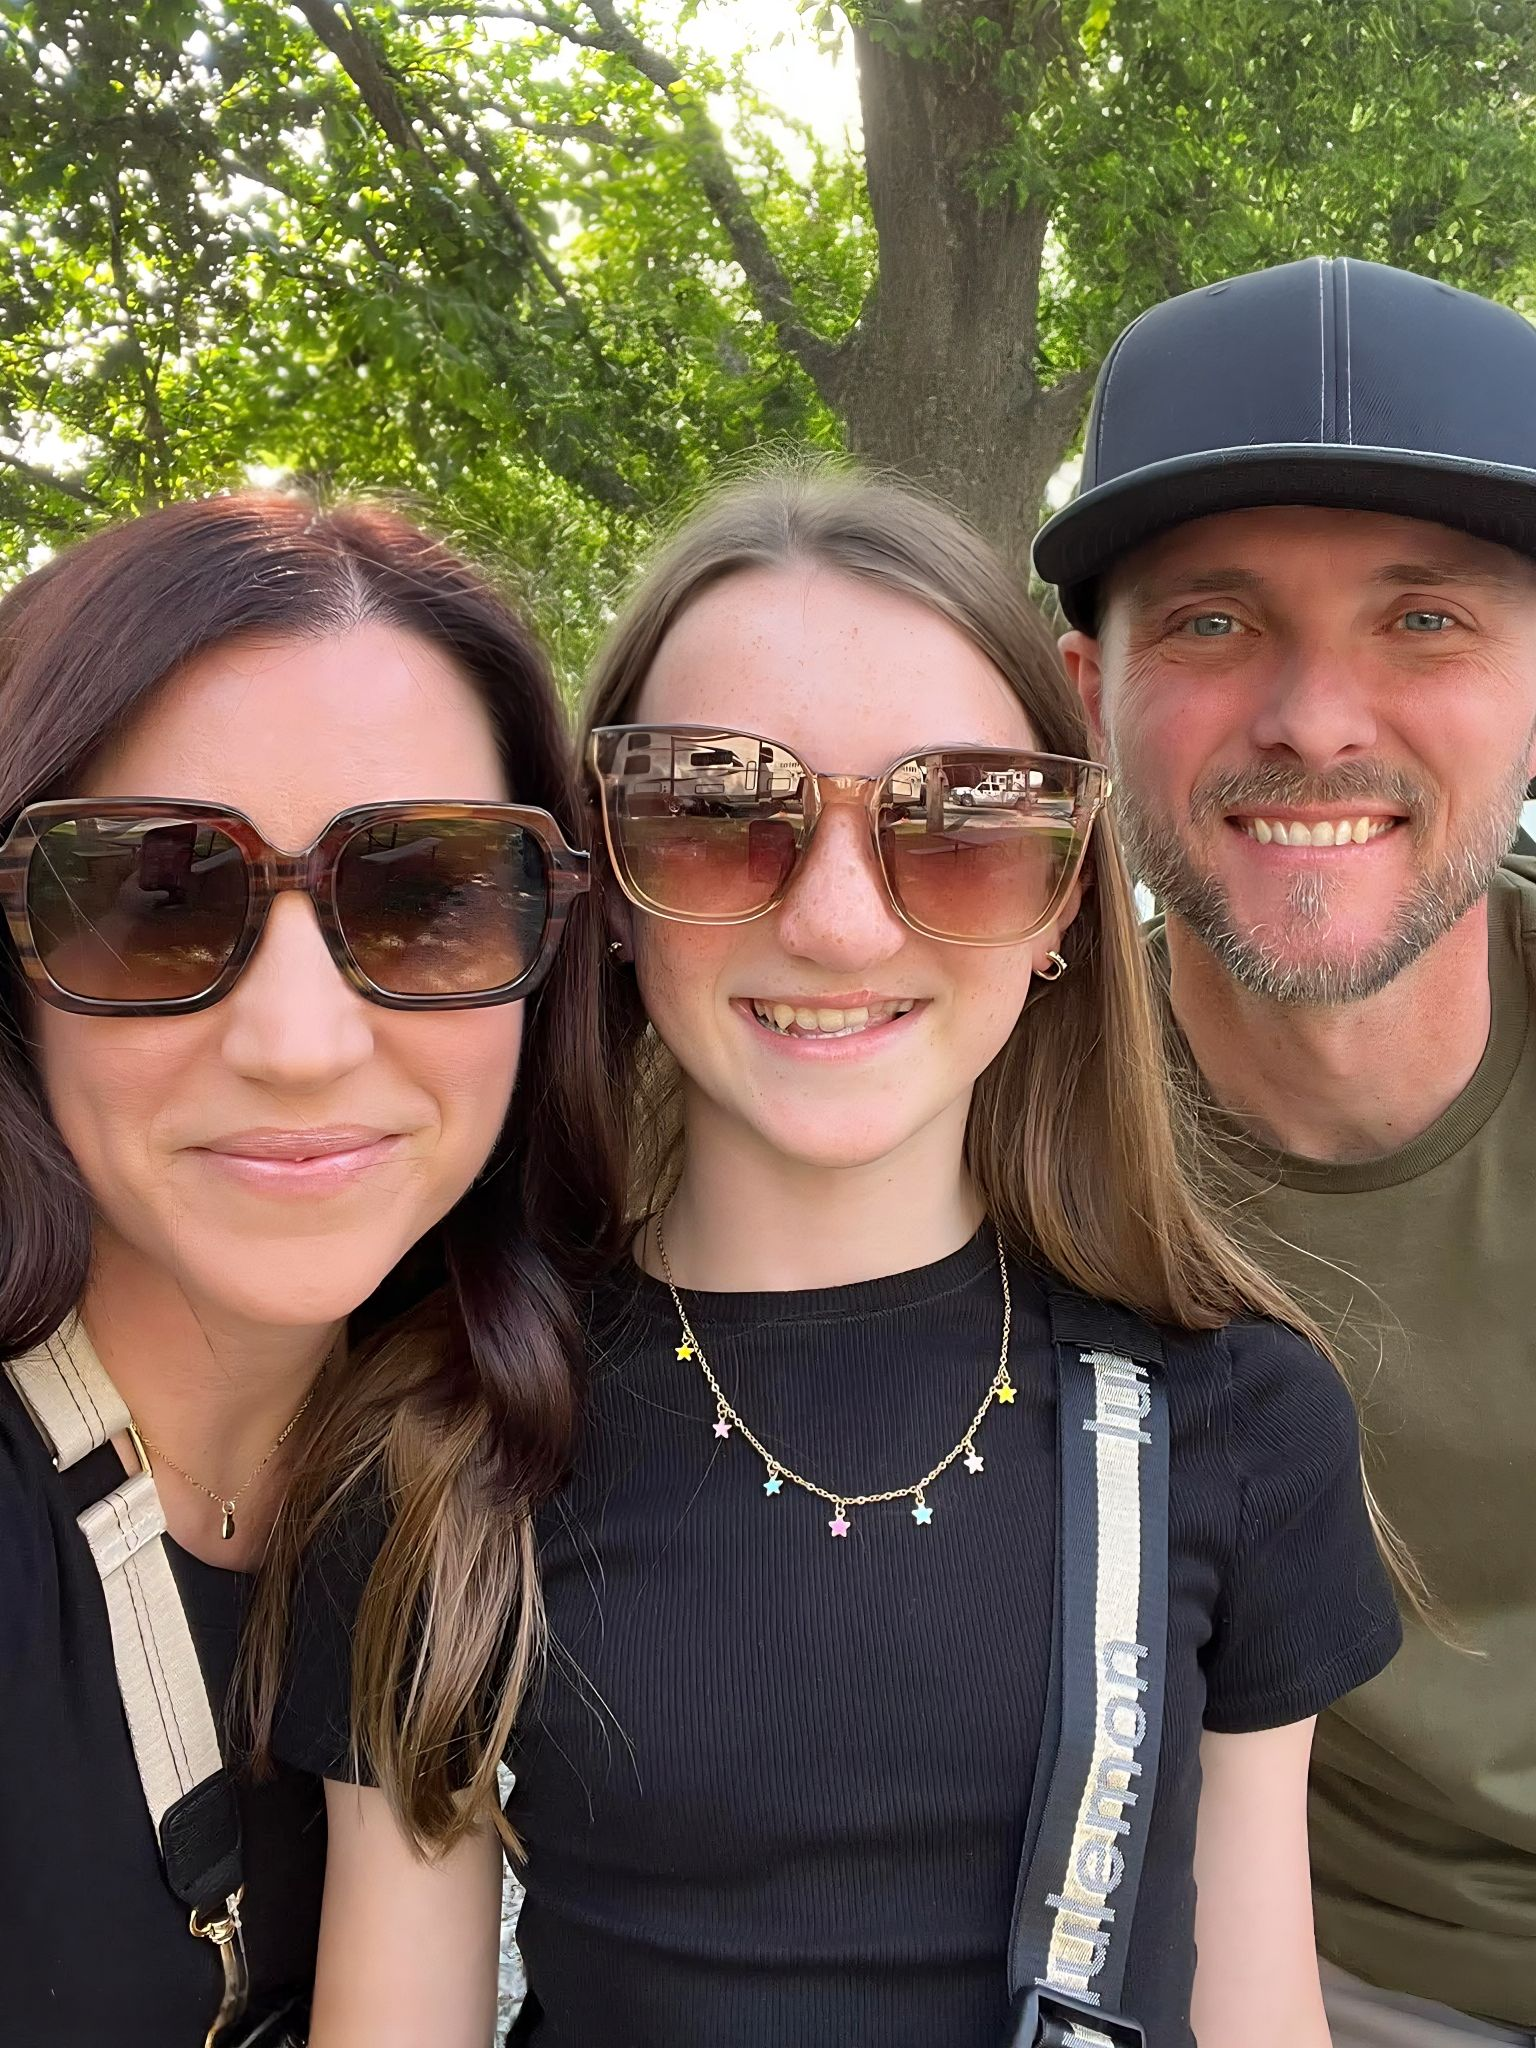
\includegraphics[width=0.3\textwidth]{images/set2/p4.jpg} \\
        set2/p3.jpg & set2/p4.jpg
    \end{tabular}
    \label{fig:set2_p3_p4}
\end{figure}

\par \textbf{set2/p3.jpg} \-- Here we have an `AI generated content' warning in the bottom left corener of the image.
This might be a clue. Also the girl's hair seems to be very well edited, I couldn't tell that this image was manipulated
based on her hair. However, the woman's hair lose a lot of details at the top, it get's blurred and the end of the hair
strands are not visible or have very low quality. This image is \textbf{manipulated}.

\par \textbf{set2/p4.jpg} \-- This image is very similar to the previous one. The girl's hair is very well edited again.
Now there is no `AI generated content' warning, but the woman's hair is again blurred at the top and the end of the hair
strands. This image is also \textbf{manipulated}.

\begin{figure}[htbp]
    \centering
    \begin{tabular}{ccc}
        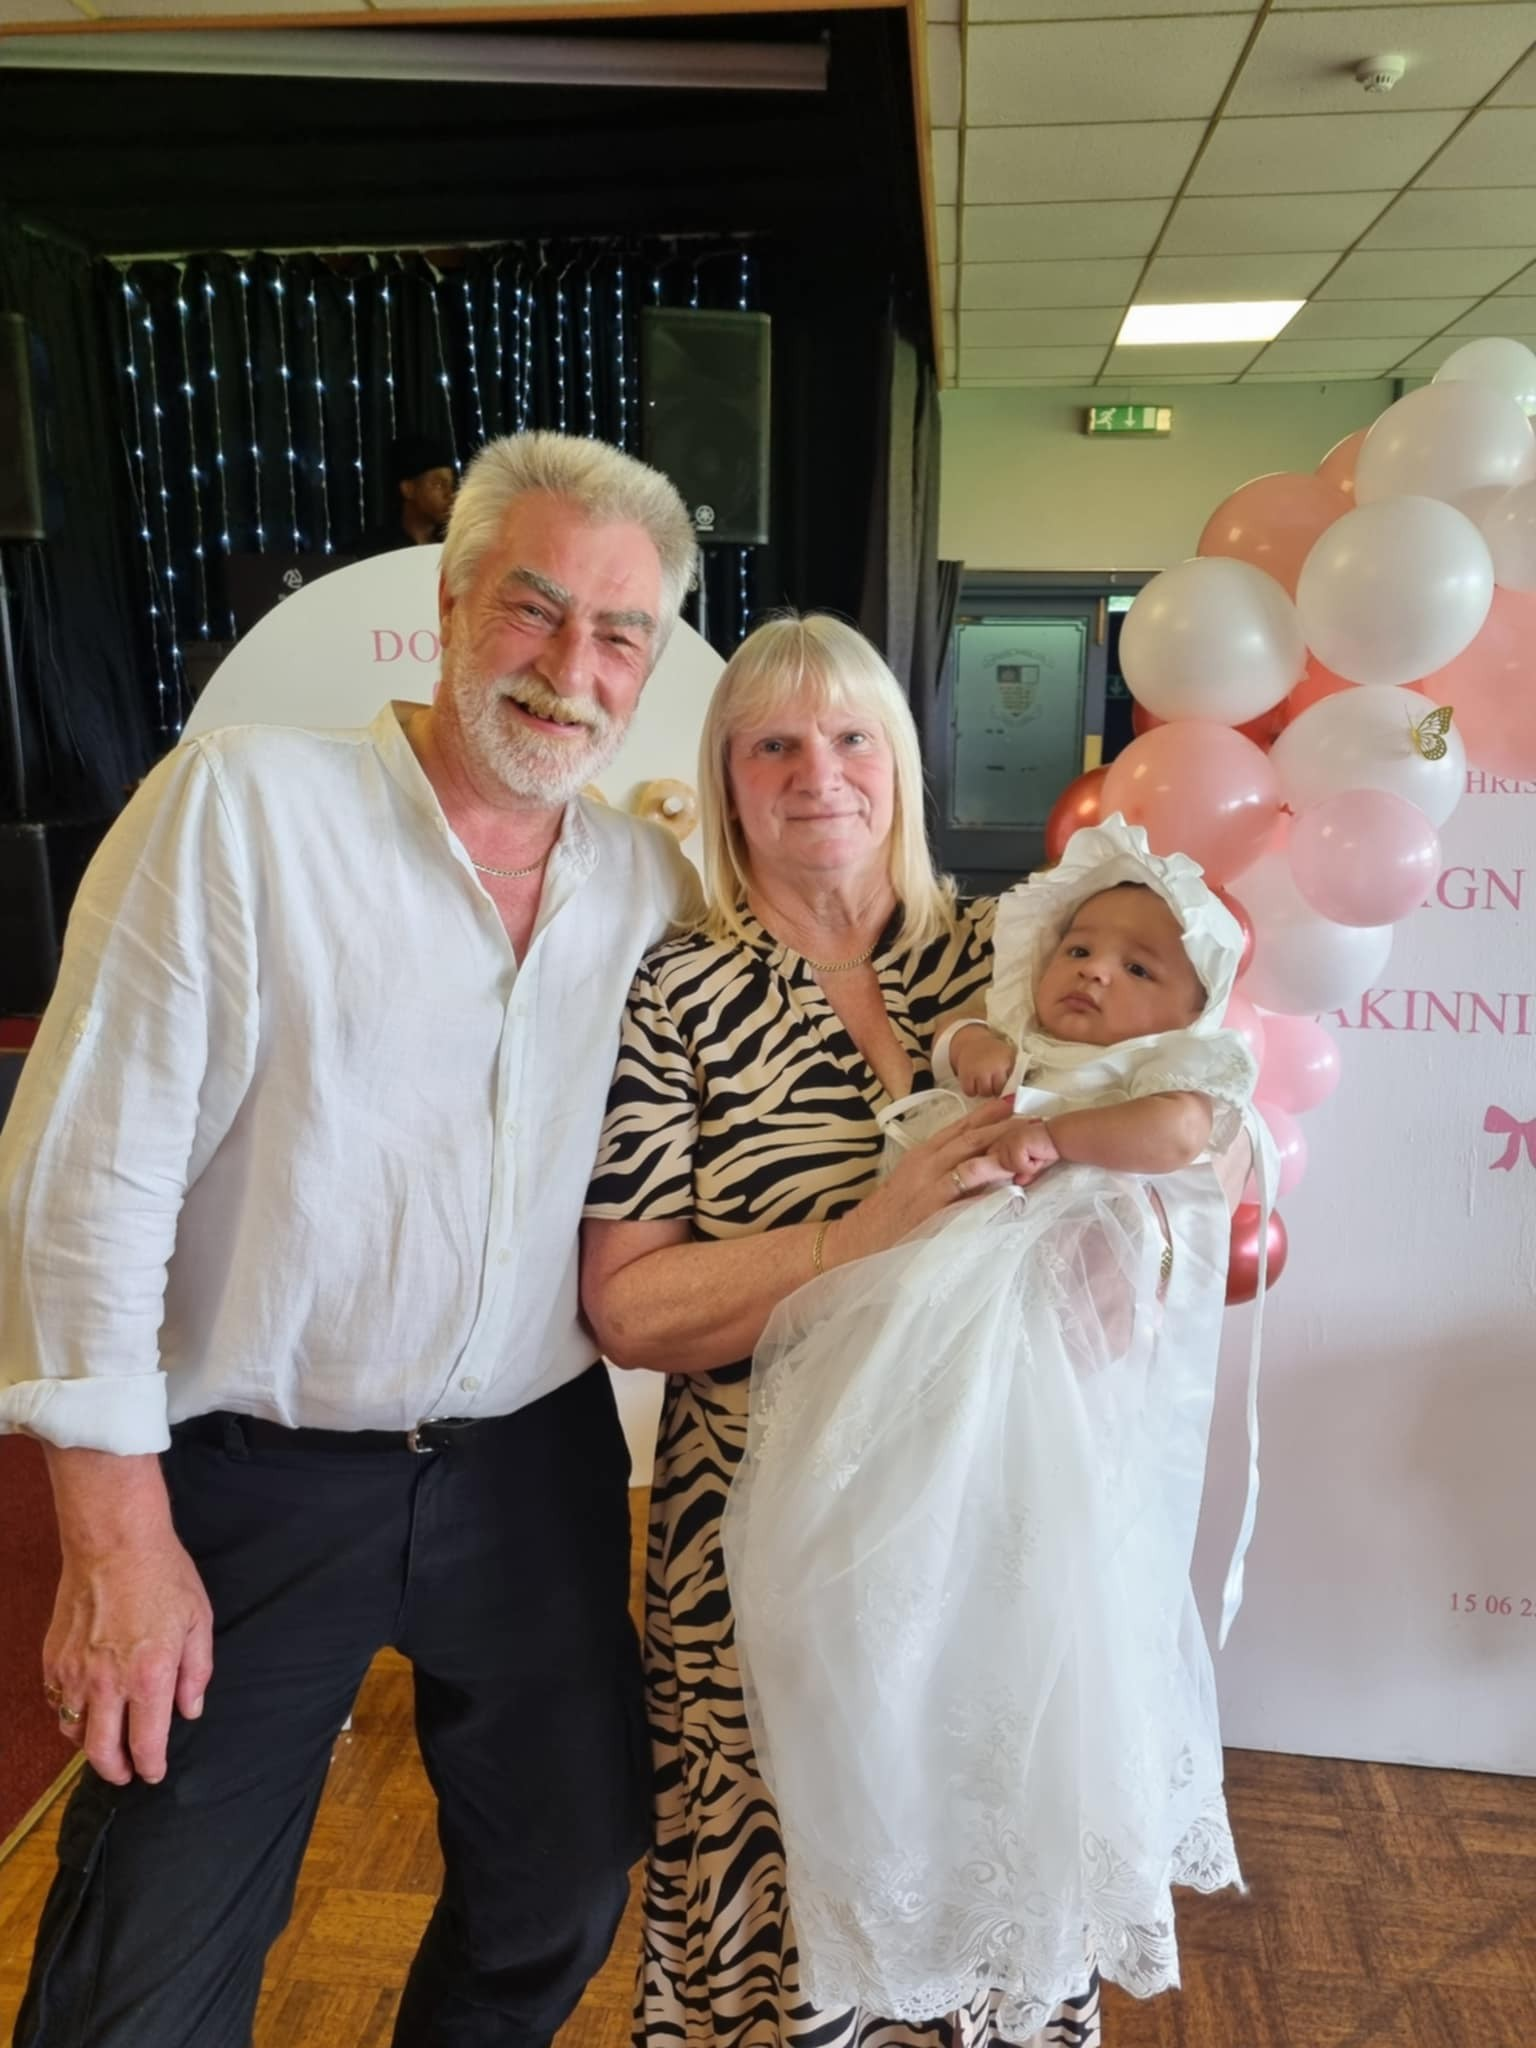
\includegraphics[width=0.3\textwidth]{images/set3/p1.jpg} &
        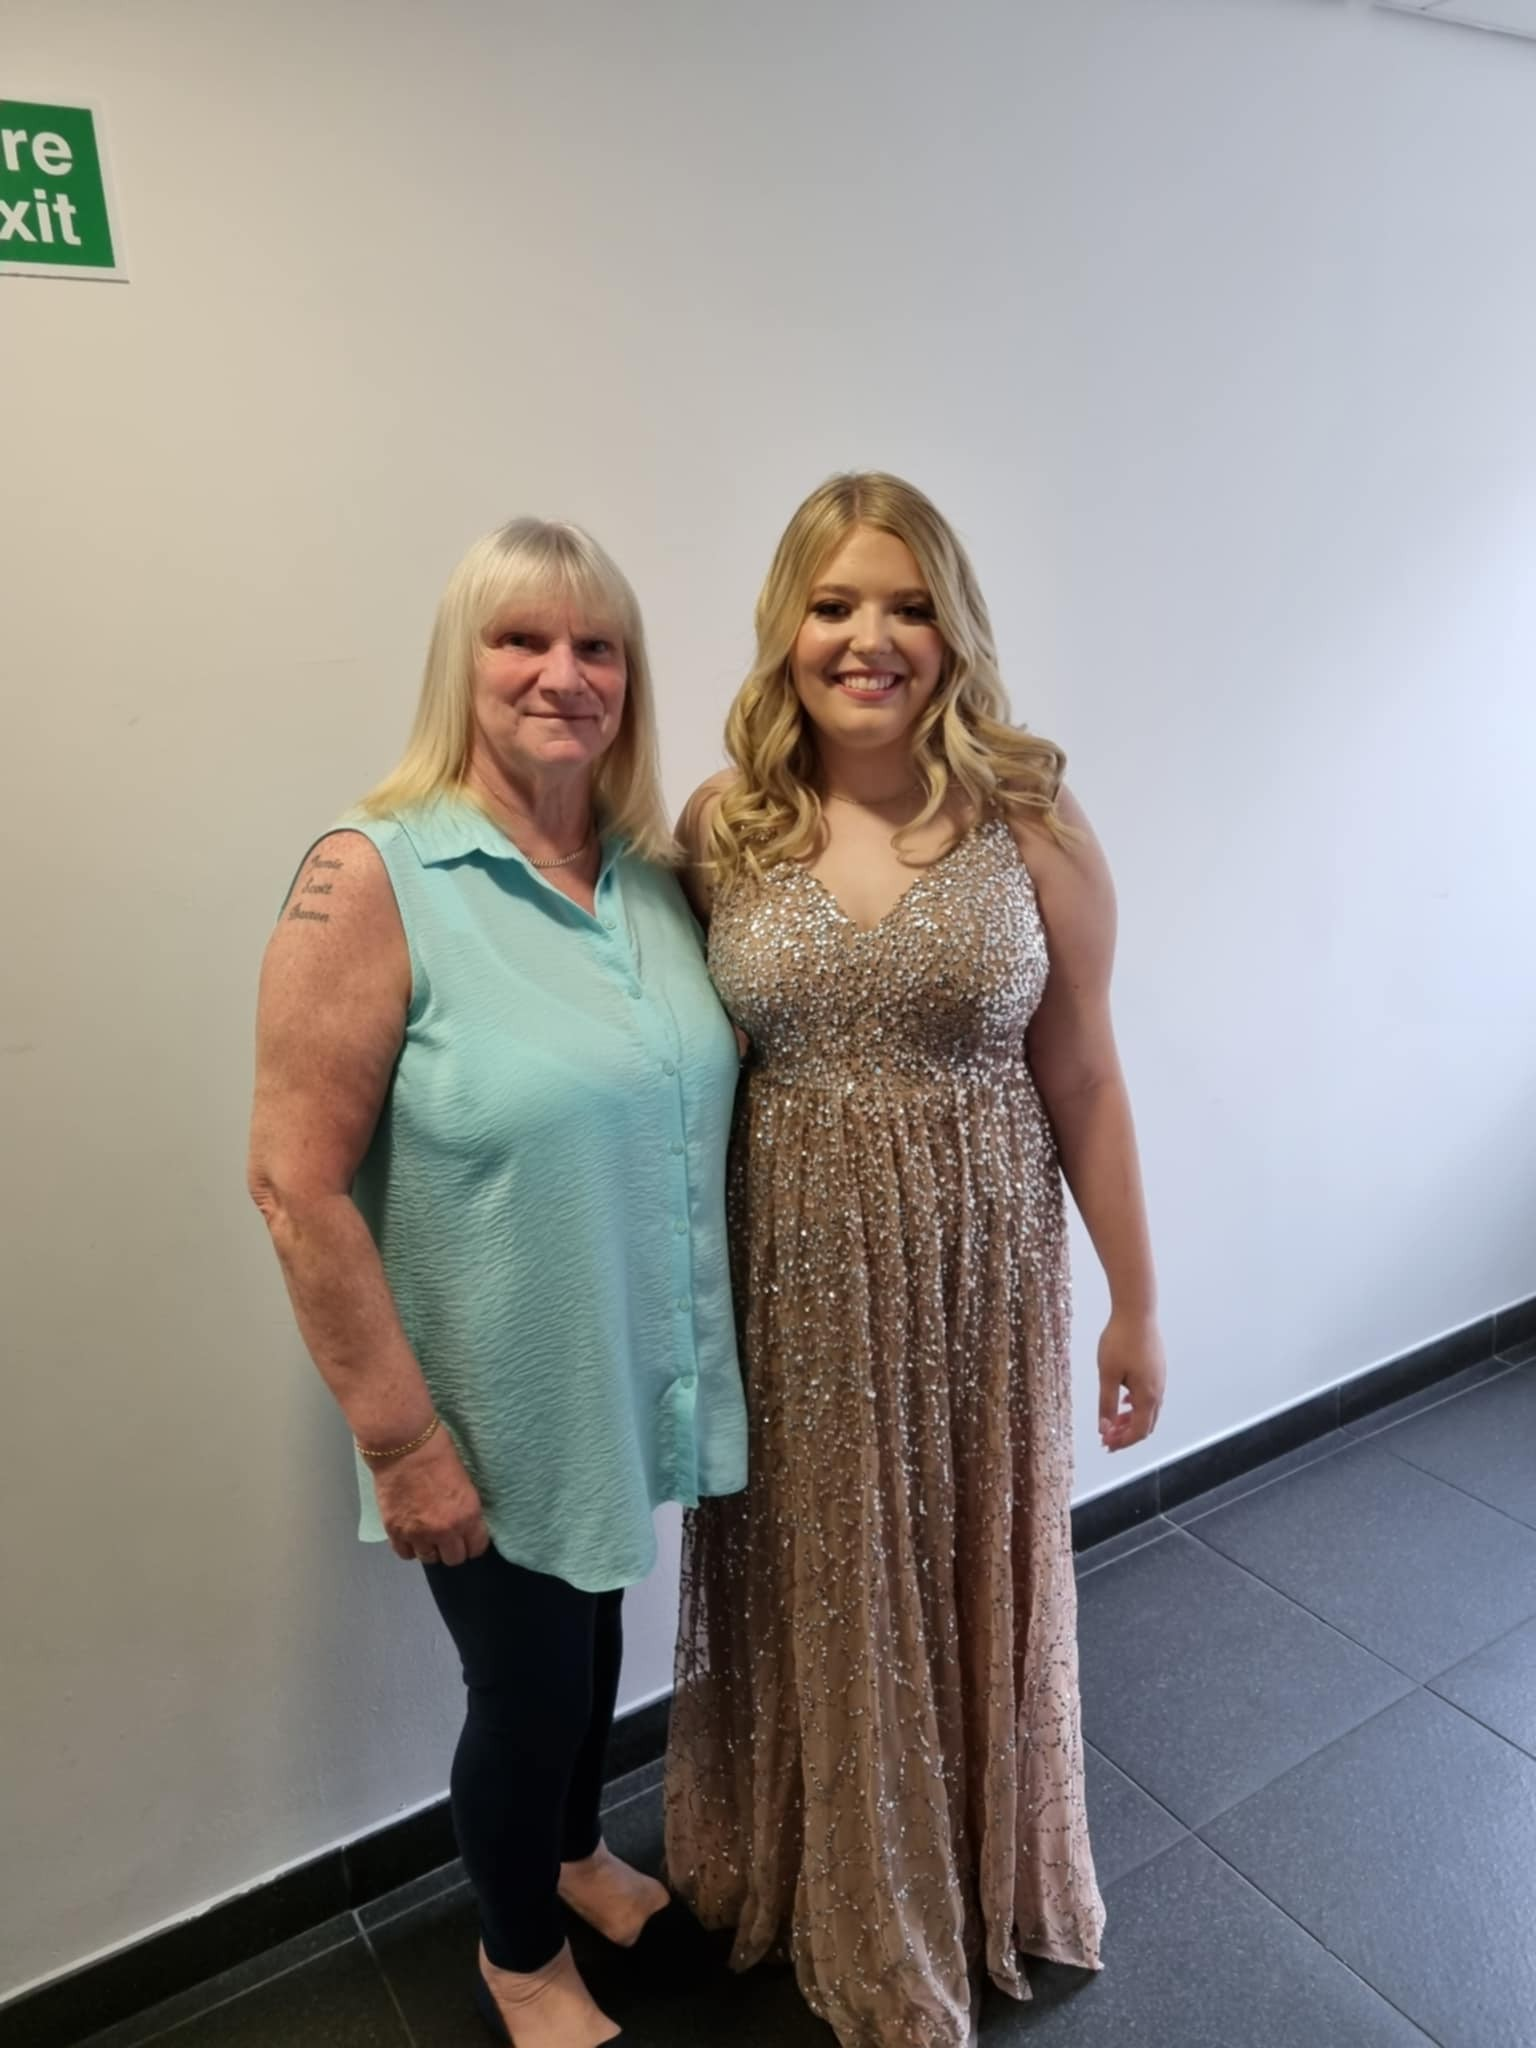
\includegraphics[width=0.3\textwidth]{images/set3/p2.jpg} &
        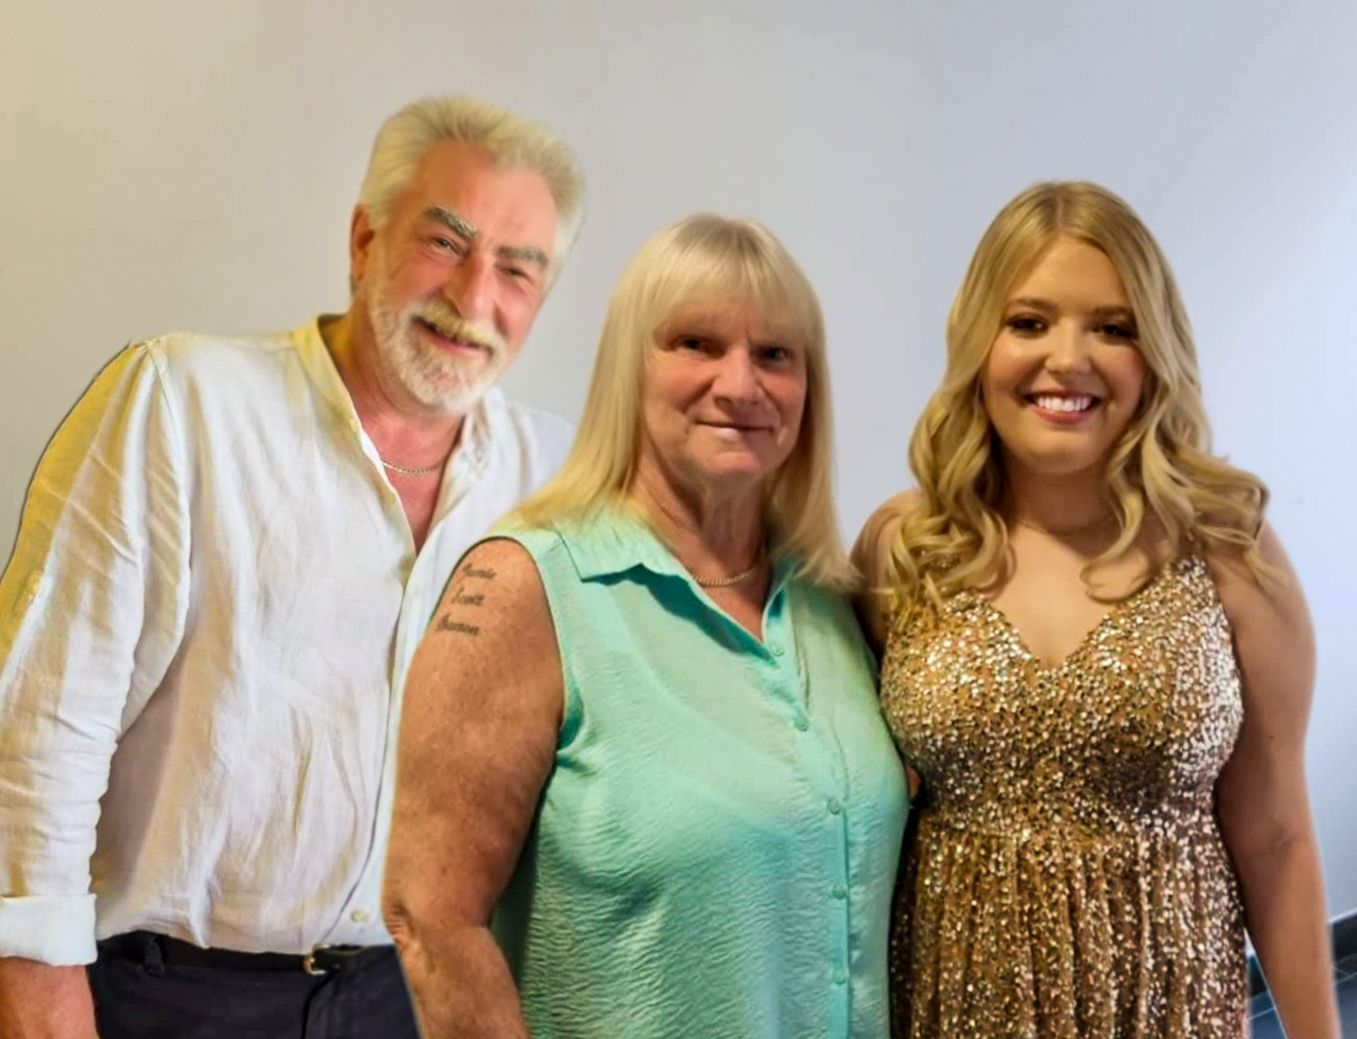
\includegraphics[width=0.3\textwidth]{images/set3/p3.jpg} \\
        set3/p1.jpg & set3/p2.jpg & set3/p3.jpg
    \end{tabular}
    \label{fig:set3_images}
\end{figure}

\par \textbf{set3/p1.jpg} \-- I can't find any inconsistencies in this image. The pixel structure is consistent, the
lighting is natural, and there are no signs of manipulation. This image is \textbf{authentic}.

\par \textbf{set3/p2.jpg} \-- The pixel structure is consistent, the lighting is natural. I can't find any signs of
manipulation. The hair strands are also consistent. This image is \textbf{authentic}.

\par \textbf{set3/p3.jpg} \-- Compared to p2.jpg, the girl's teeth are more white. However, I couldn't tell this without
comparing the two images. Also, the man it was obviously edited. The shadow it's on the left side of the women's face,
but for the man is on the right side. The line between the man and the woman is blury, unnatural and inconsistent. The
man has contours in some places. This image is \textbf{manipulated}.

\begin{figure}[H]
    \centering
    \begin{tabular}{cccc}
        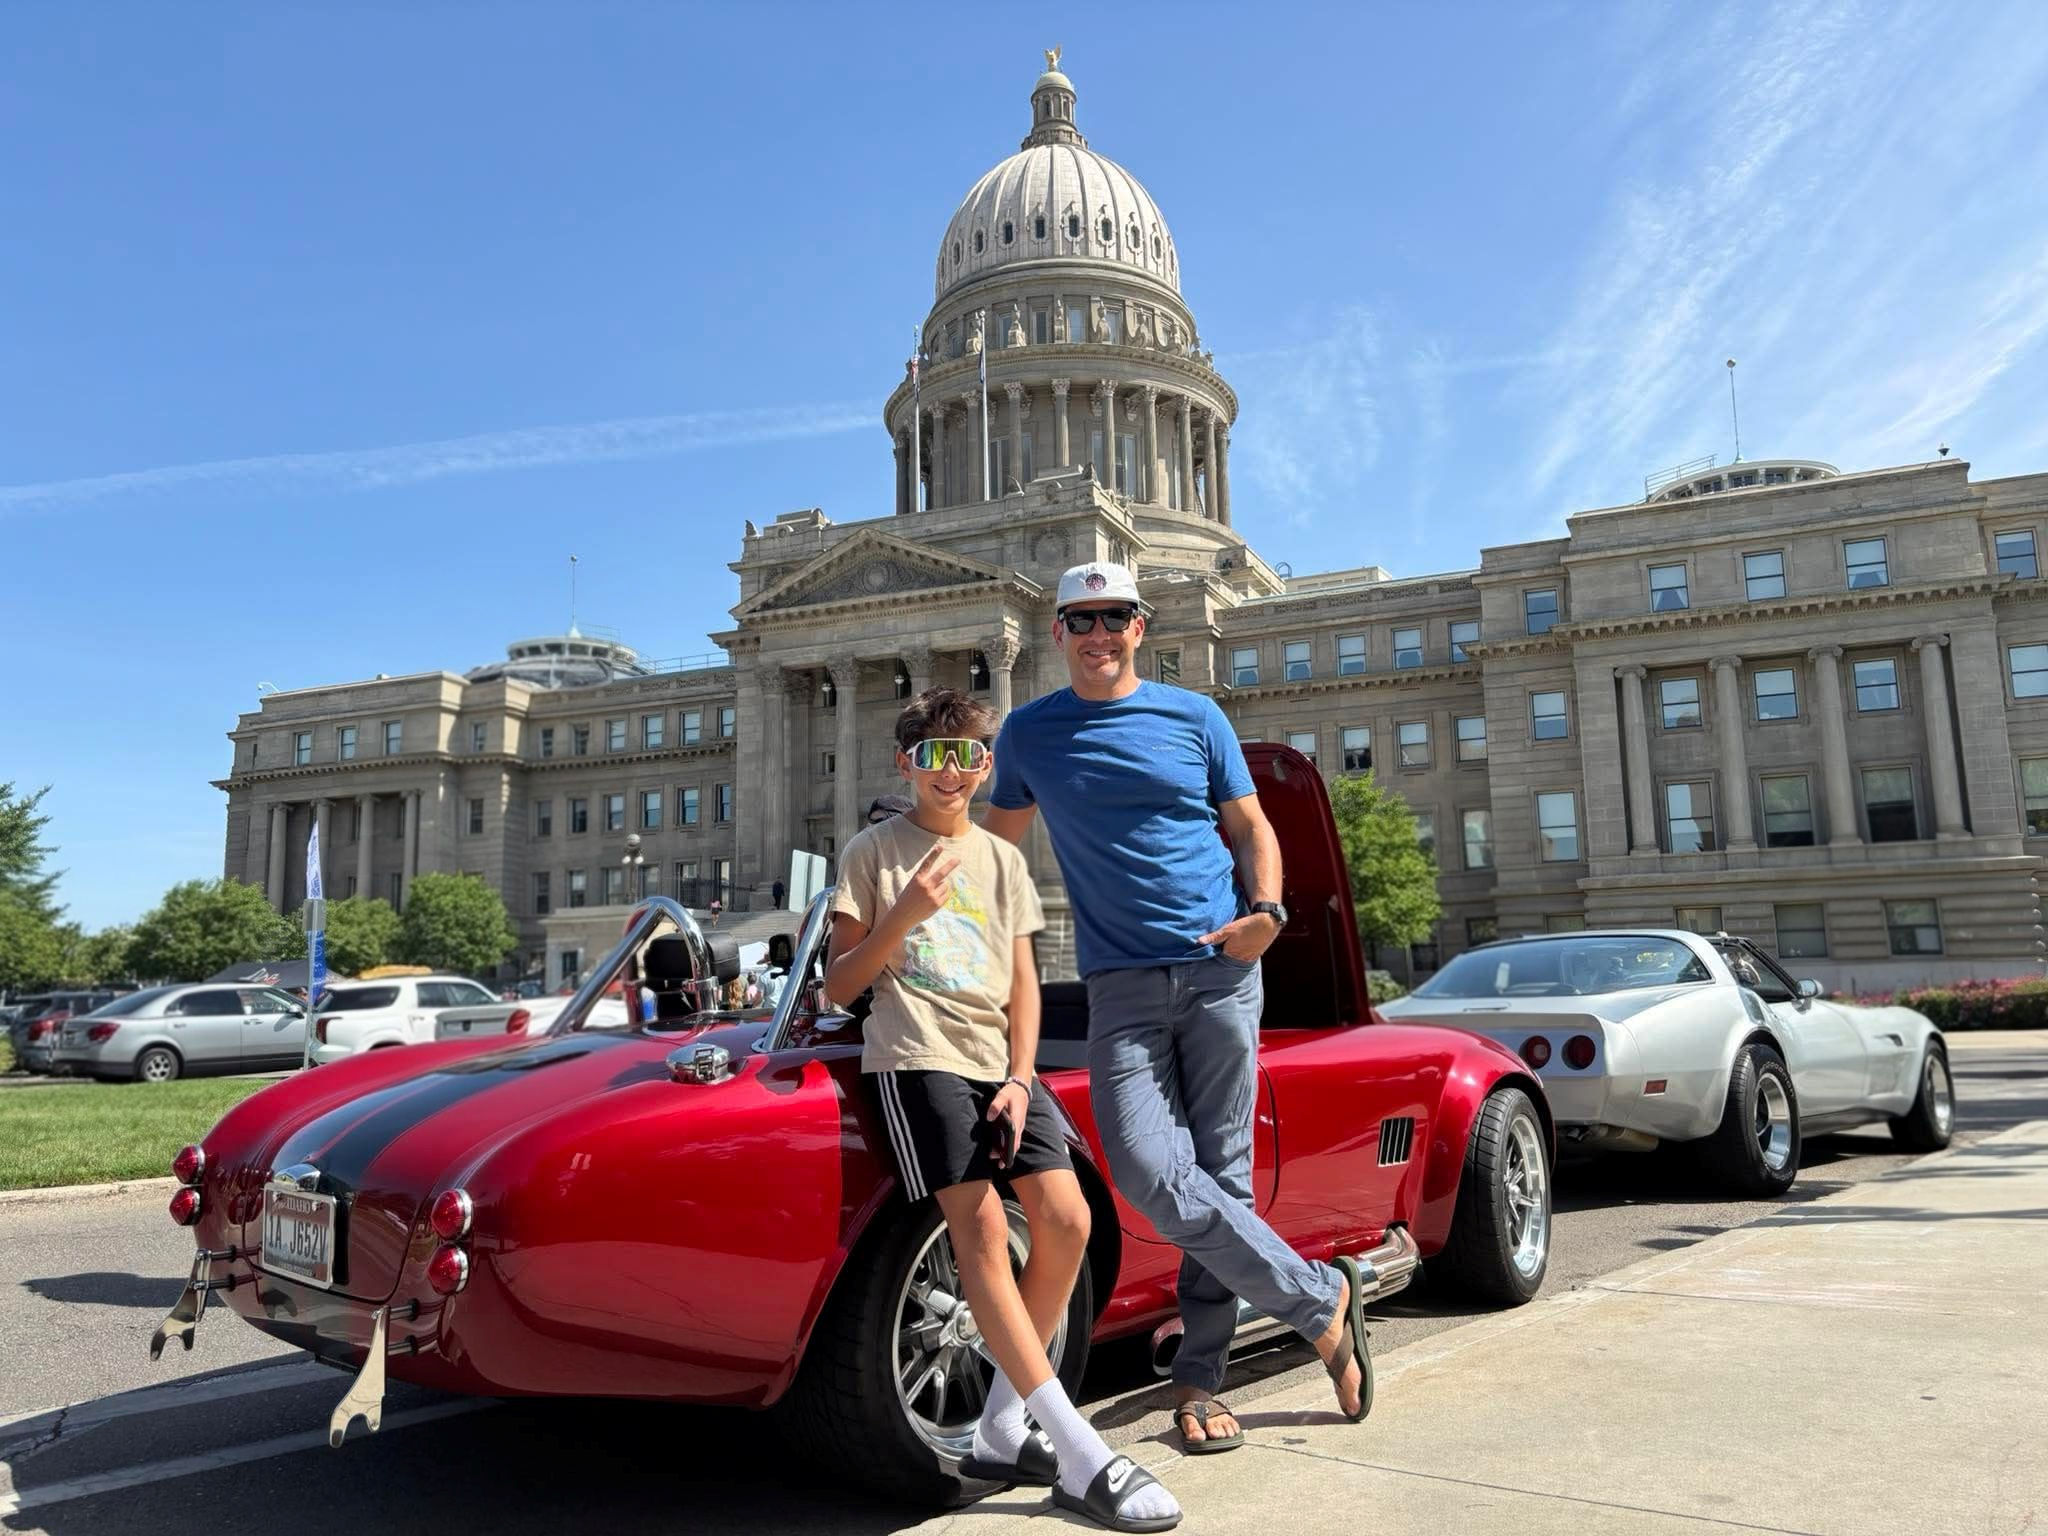
\includegraphics[width=0.45\textwidth]{images/set4/p1.jpg} &
        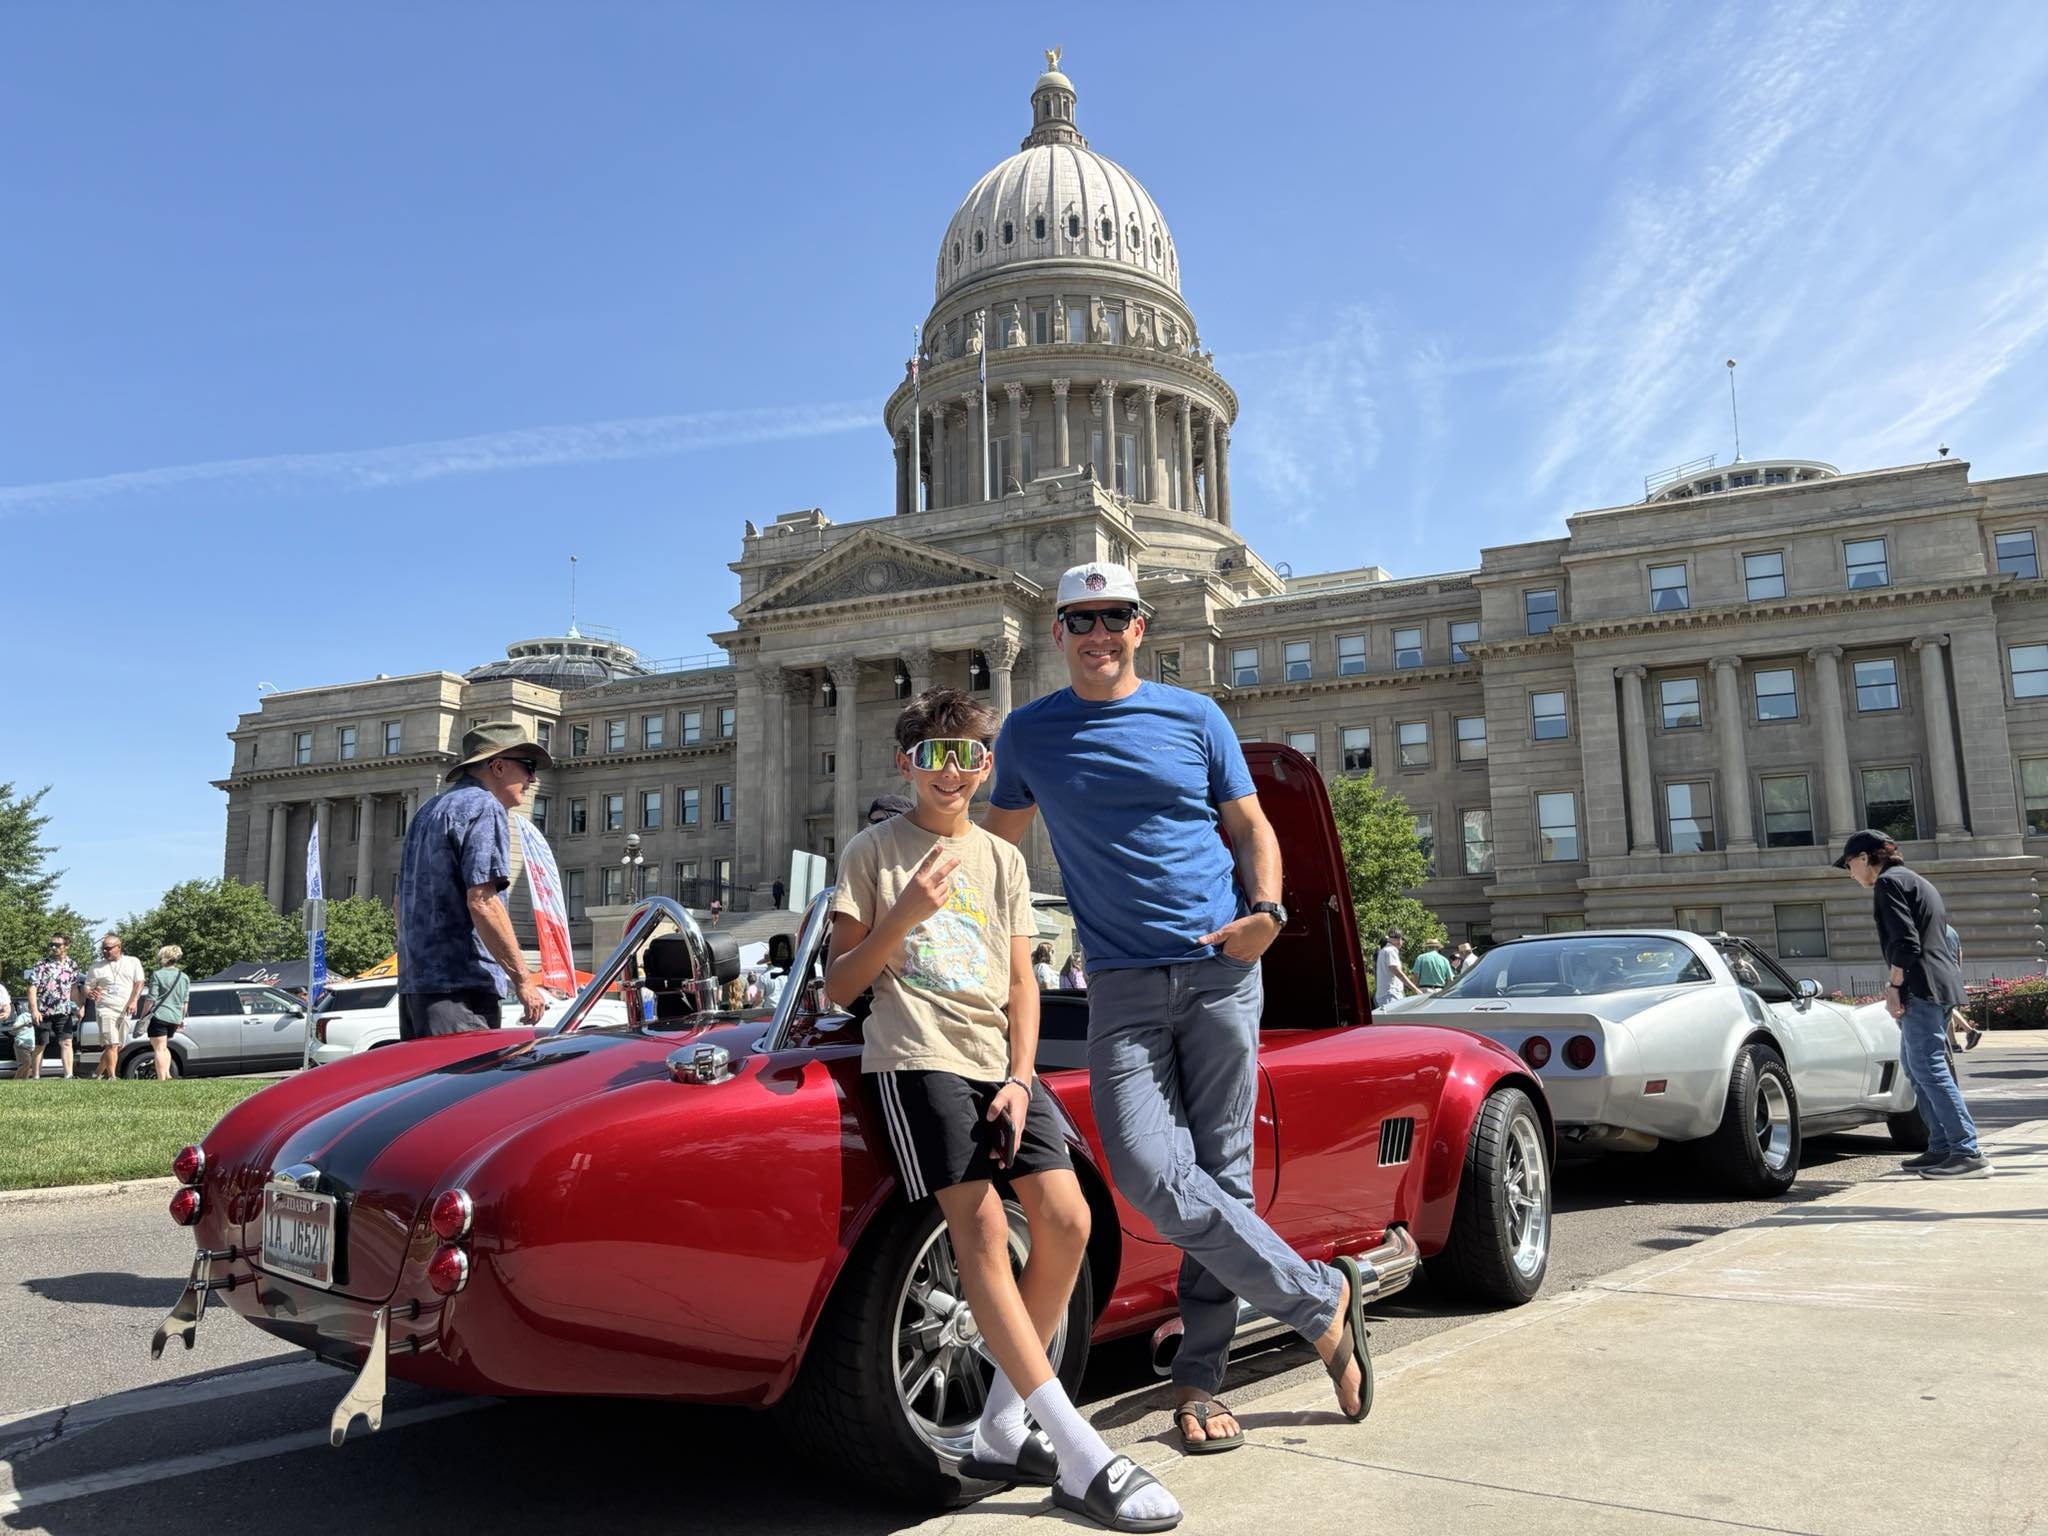
\includegraphics[width=0.45\textwidth]{images/set4/p2.jpg} \\
        set2/p4.jpg & set2/p4.jpg
    \end{tabular}
    \label{fig:set4_images}
\end{figure}

\par \textbf{set4/p1.jpg} \-- There are multiple blurry areas in this image, and the cars from the left bottom corner
seems to be distorsioned and blurred. Other blurry areas around the left tower and at the front wheel of the grey car
from right. These blurry areas are not consistent with the rest of the image. This image is \textbf{manipulated}.

\par \textbf{set4/p2.jpg} \-- Here I can't find any inconsistencies. The pixel structure is consistent, the lighting
is natural. This image is \textbf{authentic}.

\begin{figure}[htbp]
    \centering
    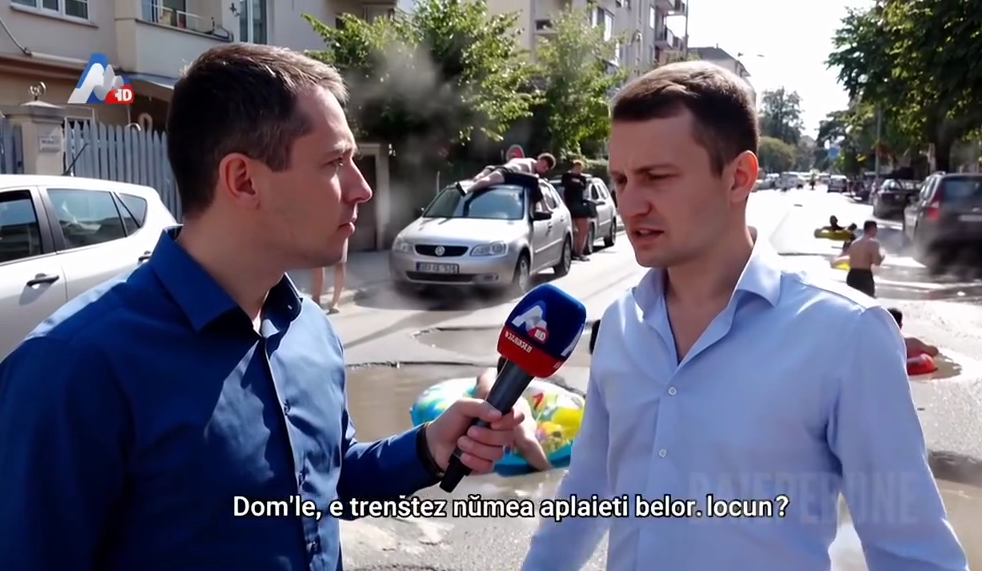
\includegraphics[width=0.6\textwidth]{images/data5_v1.png}
    \caption{video1.mp4}
    \label{fig:video1}
\end{figure}

\par In this video every text (car numbers, subtitles, etc.) is gibberish. The movement of the lips are unnatural and
the people from this video always look in strange directions, not where you would expect a person to look. For example,
there is hard to find a normal eye-contact between to people that are talking to each other. At \texttt{0:31} the man
leaving the water is not as wet as he naturally should be. The old woman's mouth at the end of the video is very
unnatural. This video is \textbf{manipulated}.

\begin{figure}[htbp]
    \centering
    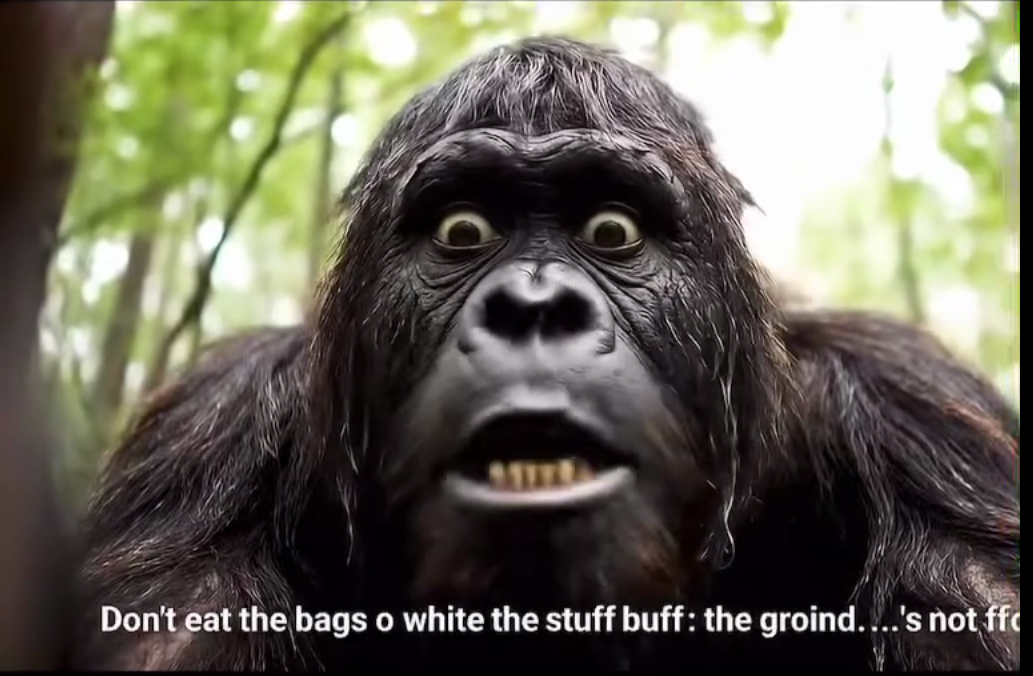
\includegraphics[width=0.6\textwidth]{images/data5_v2.png}
    \caption{video2.mp4}
    \label{fig:video2}
\end{figure}

\par In this video, the man and BigFoot are booth looking in the same direction, and both of their mouths are moving,
even if only BigFoot is talking. BigFoot. BigFoot is talking. The movement of BigFoot's mouth is unnatural. His face
is slightly blurred, and slightly different in each section. BigFoot has human-like eyes and teeth. When BigFoot bites
the "flower bag", some "flower powder" appears in his mouth from nowhere. The subtitles are gibberish. This video is
\textbf{manipulated}.

\section{Conclusion}

\par In this paper, I presented the operation CYBERSHADOW\@: A Digital Whodunit. I described each step of the
investigation, the tools and techniques used, and the results obtained.

\par The investigation started with a file type detection. I wrote a C++ script that recursively scans a directory
and identifies the actual file type for each file based on the magic number of the file's header.

\par The next step was to analyze the network traffic logs. I used Wireshark to visualize the traffic and extract the
relevant information. Here it was necessarry to look for patterns and suspicious traffic.

\par The third step was to analyze the USB image. I mounted the image and extracted the files. I also decrypted an
encrypted file using a brute-force approach. I used the `file' command to identify the file types and `binwalk' to
deep scan the files. I also used `exiftool' and `steghide' to extract the metadata and hidden data from the image files.

\par The last step was to analyze the media files. I used a combination of manual analysis and tools to determine
which images and videos were authentic and which had been manipulated. I looked for pixel structure anomalies, metadata
and lighting inconsistencies, thin details such as hair strands, and other signs of manipulation.

%\bibliographystyle{sn-mathphys}
\bibliography{sn-bibliography}

\end{document}

